\blankpage

\pagestyle{hedra}
\label{hedra}
%\begin{textblock*}{5.625in}(0pt,0pt)%
%\vspace*{-3.5cm}
%\hspace*{-2.77cm}\includegraphics*[width=175.2mm]{./propagandas/HEDRA.pdf}
%\end{textblock*}
%\pagebreak

% \begin{center}
% \hspace*{-3.6cm}\raisebox{5cm}{\rotatebox[origin=t]{90}{\huge\textbf{Lançamento}}}
% \hspace*{3.1cm}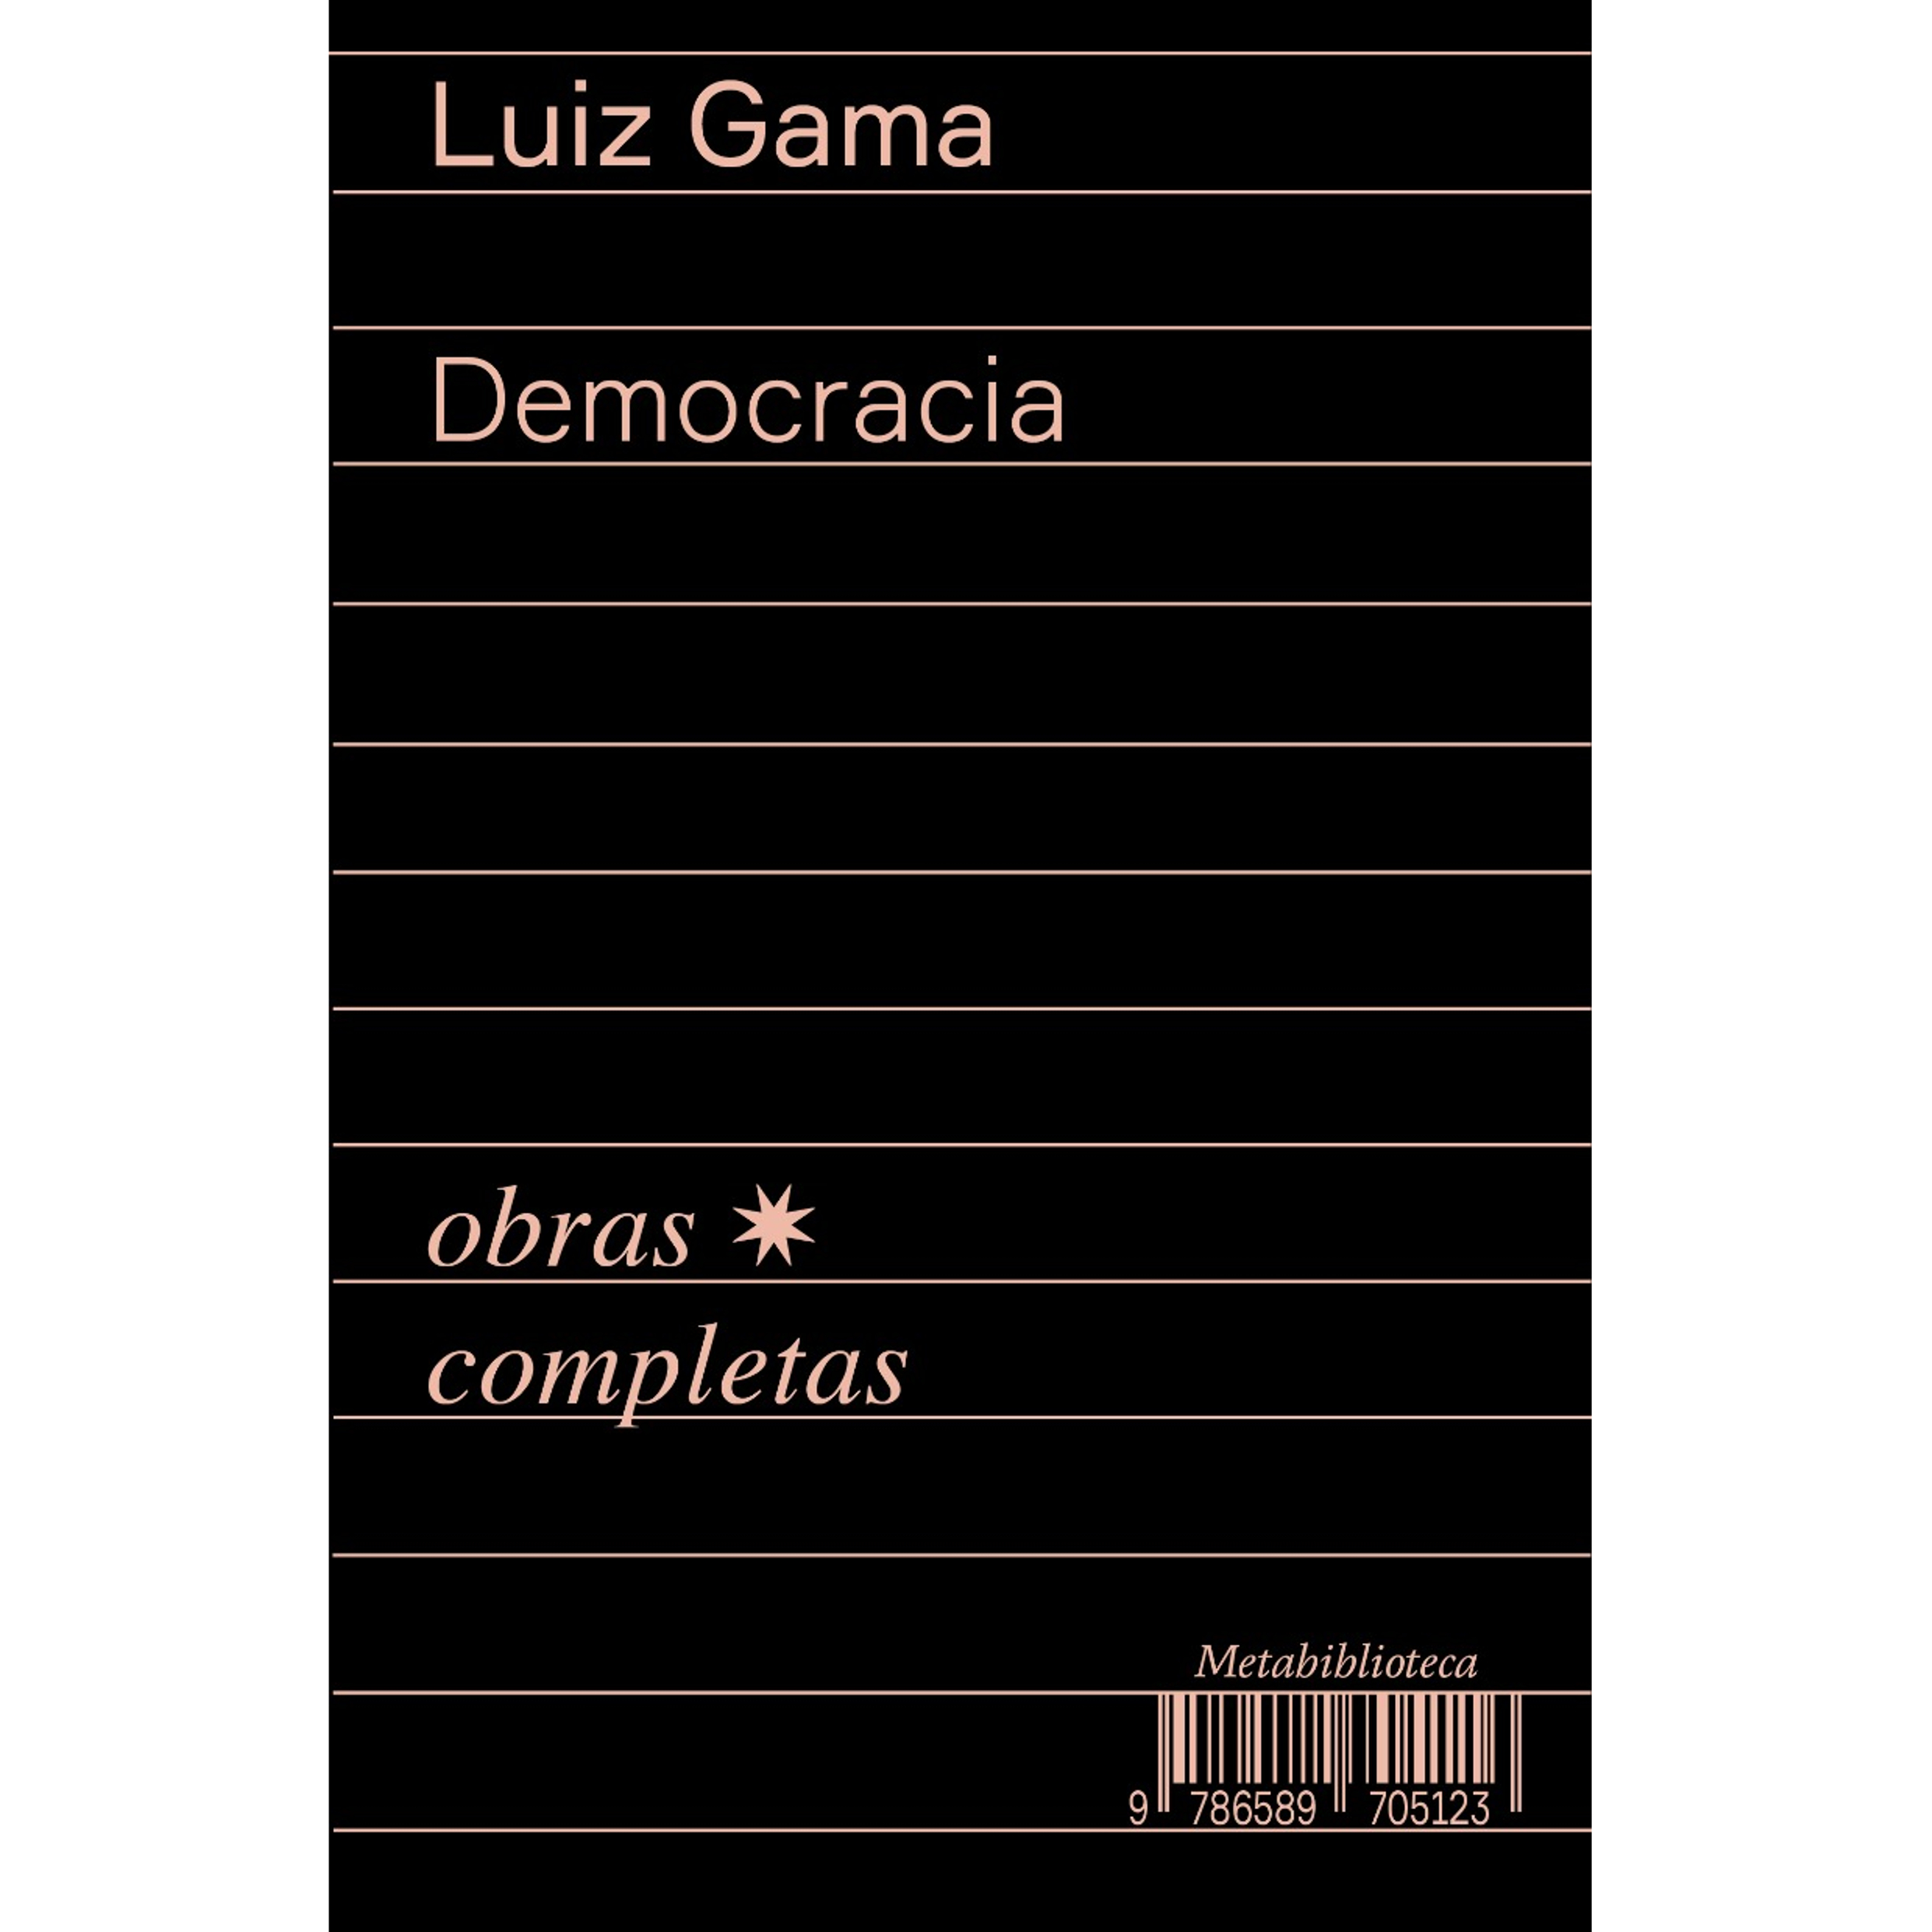
\includegraphics[width=74mm]{./CAPAS/HEDRA_DEMOCRACIA.jpg}
% \end{center}
% \hspace*{-7cm}\hrulefill\hspace*{-7cm}
% \medskip

% \noindent{}Os textos e artigos incluídos em \textit{Democracia} foram publicados originalmente entre os anos de 1866 e 1869. Nesses artigos, Luiz Gama se manifesta publicamente sobre educação, política e direitos universais. \hlc{Lançando mão de uma estratégia autoral ousada, que incluía o uso de pseudônimos, Gama defende abertamente o direito à educação universal e as obrigações do Estado em garantir um ensino público de qualidade} em todos os níveis como os fundamentos da vida democrática.

% \textit{Democracia} integra as \textit{Obras completas} de Luiz Gama, advogado negro e abolicionista, a serem lançadas em 11 volumes com cerca de 800 escritos --- 600 inéditos ---, revelando as diversas facetas e estilos empregados pelo escritor para advogar pela grande causa de sua vida: a abolição da escravidão e a emancipação negra. Esquecidos em parte por quase dois séculos, os textos foram recuperados pelo pesquisador Bruno Rodrigues de Lima, que passou nove anos localizando-os em arquivos da imprensa e do judiciário de todo o país.

% \vfill
% \noindent\begin{minipage}[c]{1\linewidth}
% {\small\textbf{
% \hspace*{-.1cm}Editora: Hedra\\
% Título: Democracia (1866--1869)\\
% Autor: Luiz Gama\\ 
% ISBN: 978-65-89705-12-3\\
% Páginas: 506\\
% Formato: 13,3x21\,cm\\
% Preço: R\$ 110,00\\
% }}
% \end{minipage}
% \pagebreak

% \begin{center}
% \hspace*{.5cm}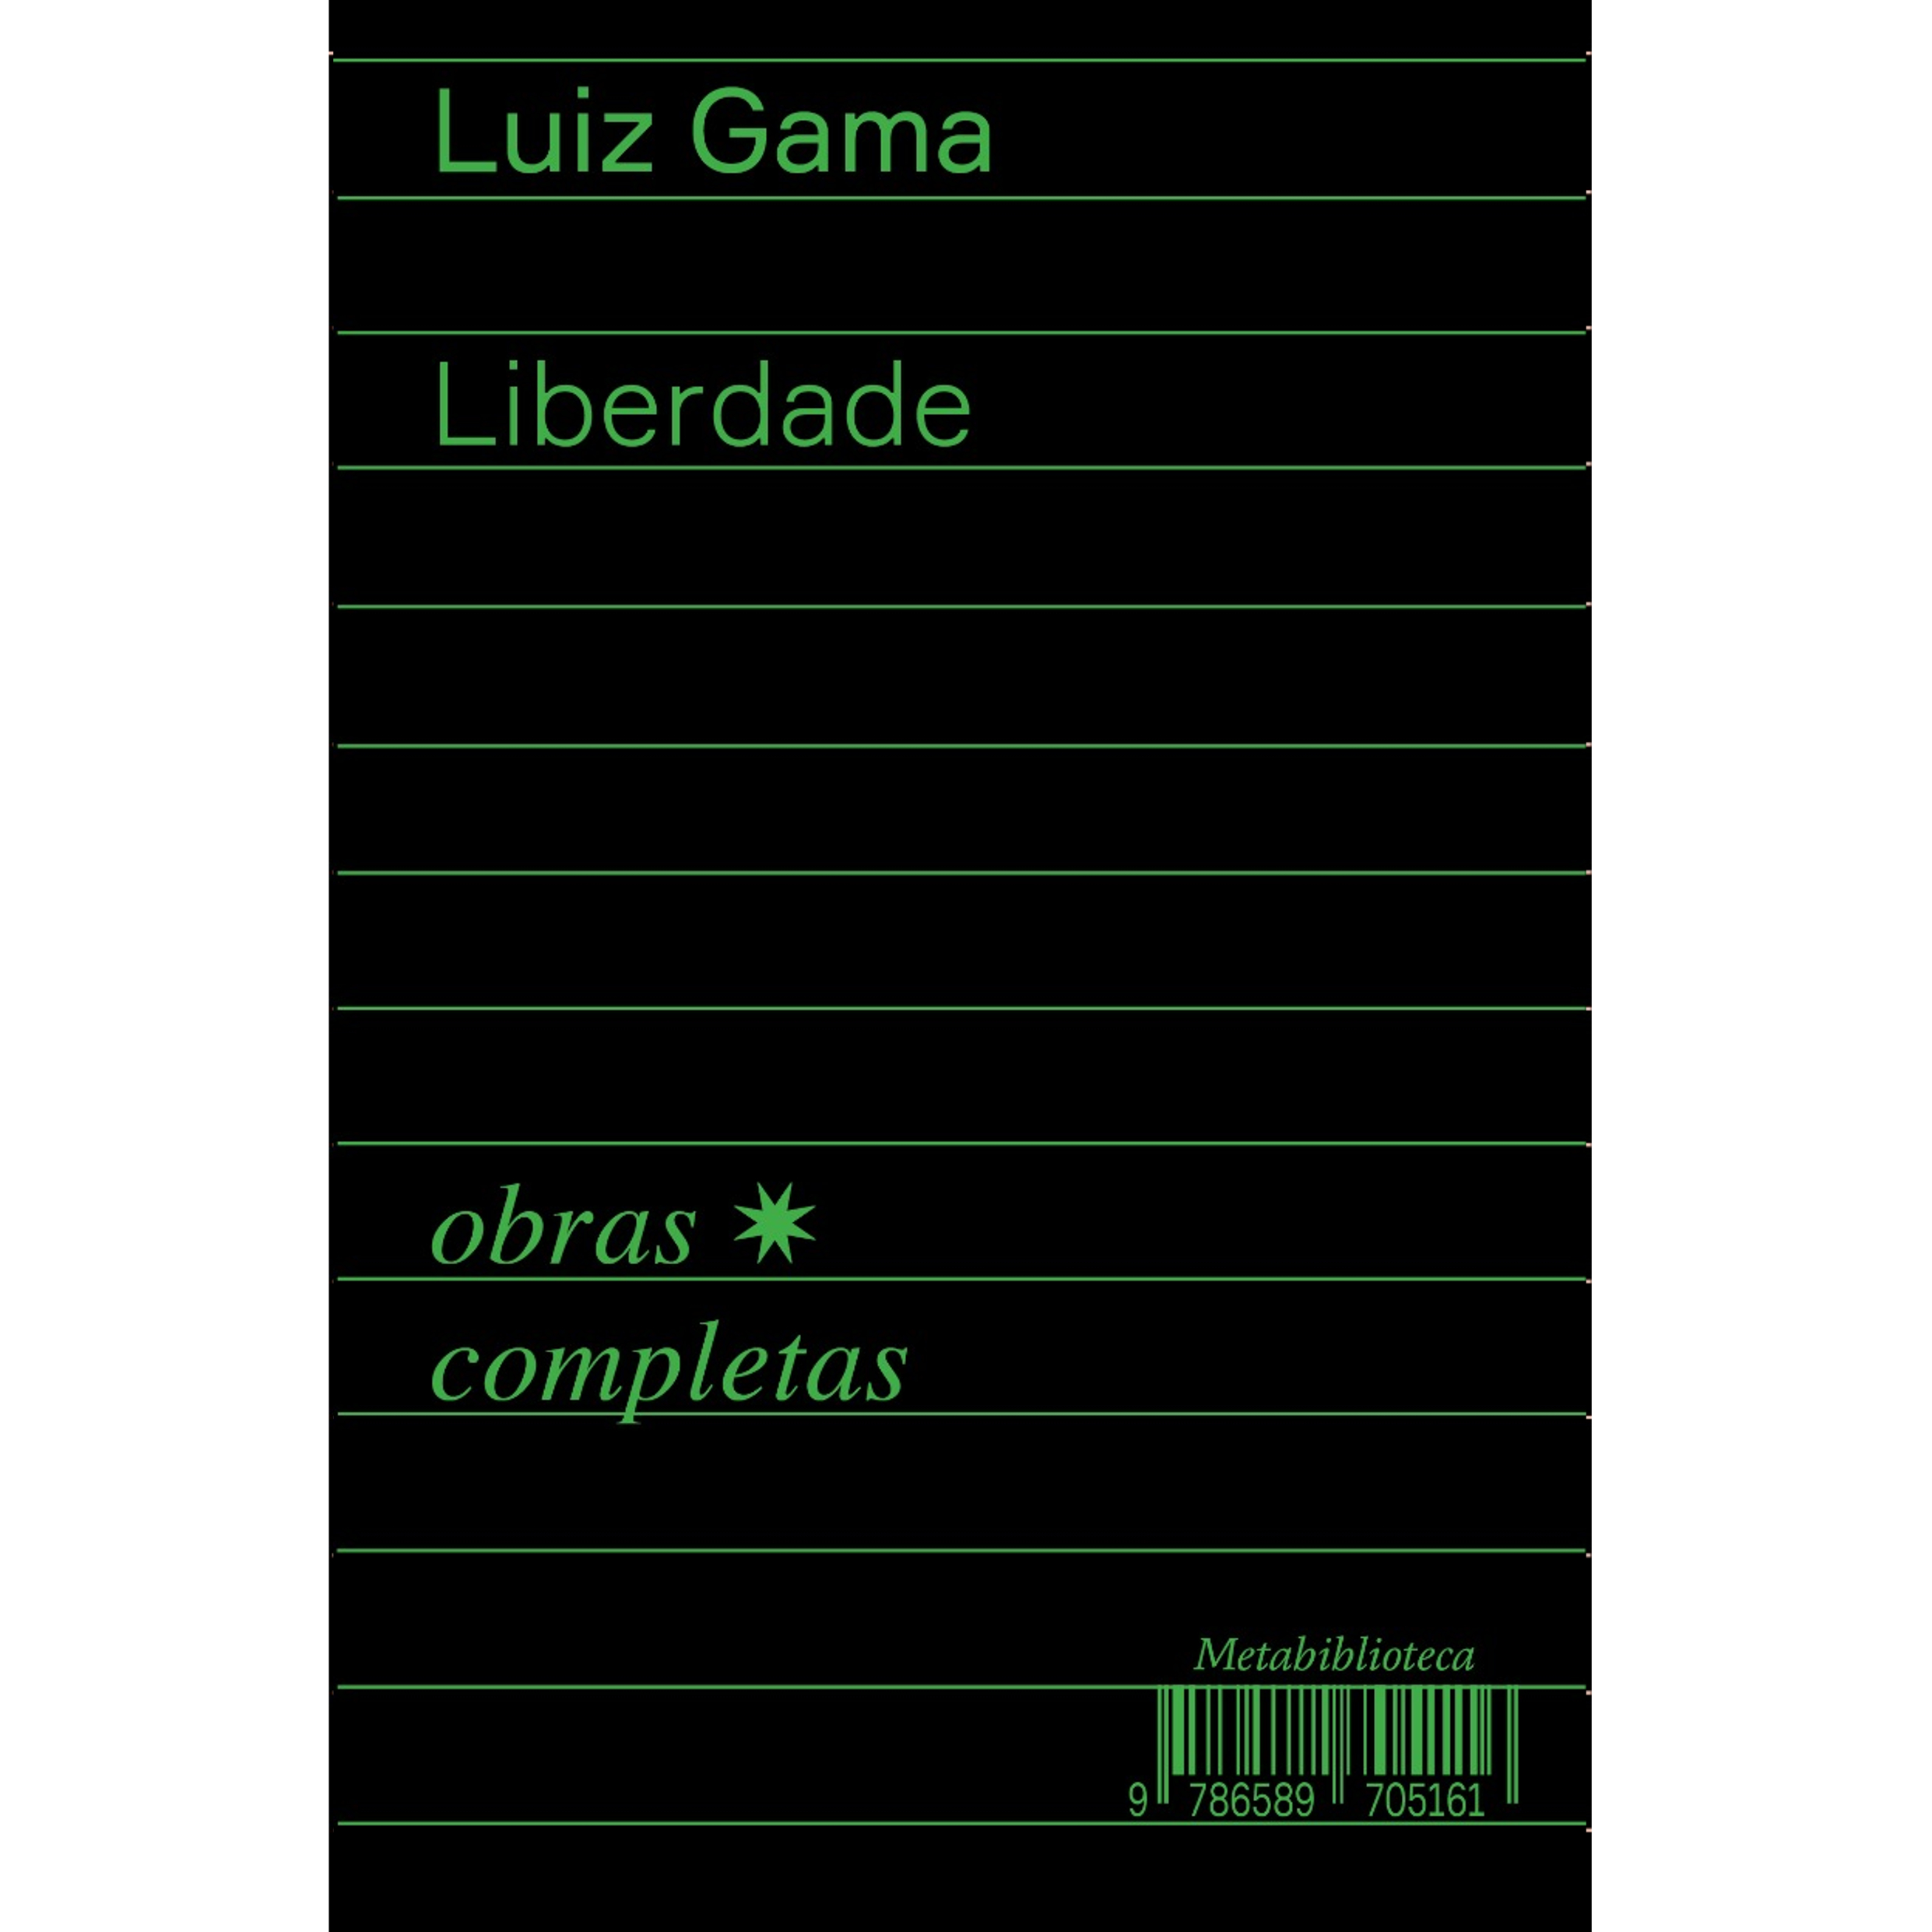
\includegraphics[width=74mm]{./CAPAS/HEDRA_LIBERDADE.jpg}
% \end{center}
% \hspace*{-7cm}\hrulefill\hspace*{-7cm}
% \medskip

% \noindent{}Os textos deste volume são \hlc{fruto da campanha pela abolição radical, que também visava à garantia da educação e cidadania para os libertos: o abolicionismo de Gama exigia cidadania e igualdade de fato e de direito}. O advogado também refletia sobre o processo histórico em curso, e propunha soluções políticas para o tempo presente, revelando sua natureza intelectual até hoje pouco conhecida e quase sempre não reconhecida.

% \textit{Liberdade} integra as \textit{Obras completas} de Luiz Gama, advogado negro e abolicionista, a serem lançadas em 11 volumes com cerca de 800 escritos --- 600 inéditos ---, revelando as diversas facetas e estilos empregados pelo escritor para advogar pela grande causa de sua vida: a abolição da escravidão e a emancipação negra. Esquecidos em parte por quase dois séculos, os textos foram recuperados pelo pesquisador Bruno Rodrigues de Lima, que passou nove anos localizando-os em arquivos da imprensa e do judiciário de todo o país.

% \vfill
% \noindent\begin{minipage}[c]{.5\linewidth}
% {\small\textbf{
% \hspace*{-.1cm}Editora: Hedra\\
% Título: Liberdade (1880--1882)\\
% Autor: Luiz Gama\\ 
% ISBN: 978-65-89705-16-1\\
% Páginas: 446\\
% Formato: 13,3x21\,cm\\
% Preço: R\$ 99,90\\
% }}
% \end{minipage}
% \pagebreak

% \begin{center}
% \hspace*{-3.6cm}\raisebox{5cm}{\rotatebox[origin=t]{90}{\huge\textbf{Lançamento}}}
% \hspace*{3.1cm}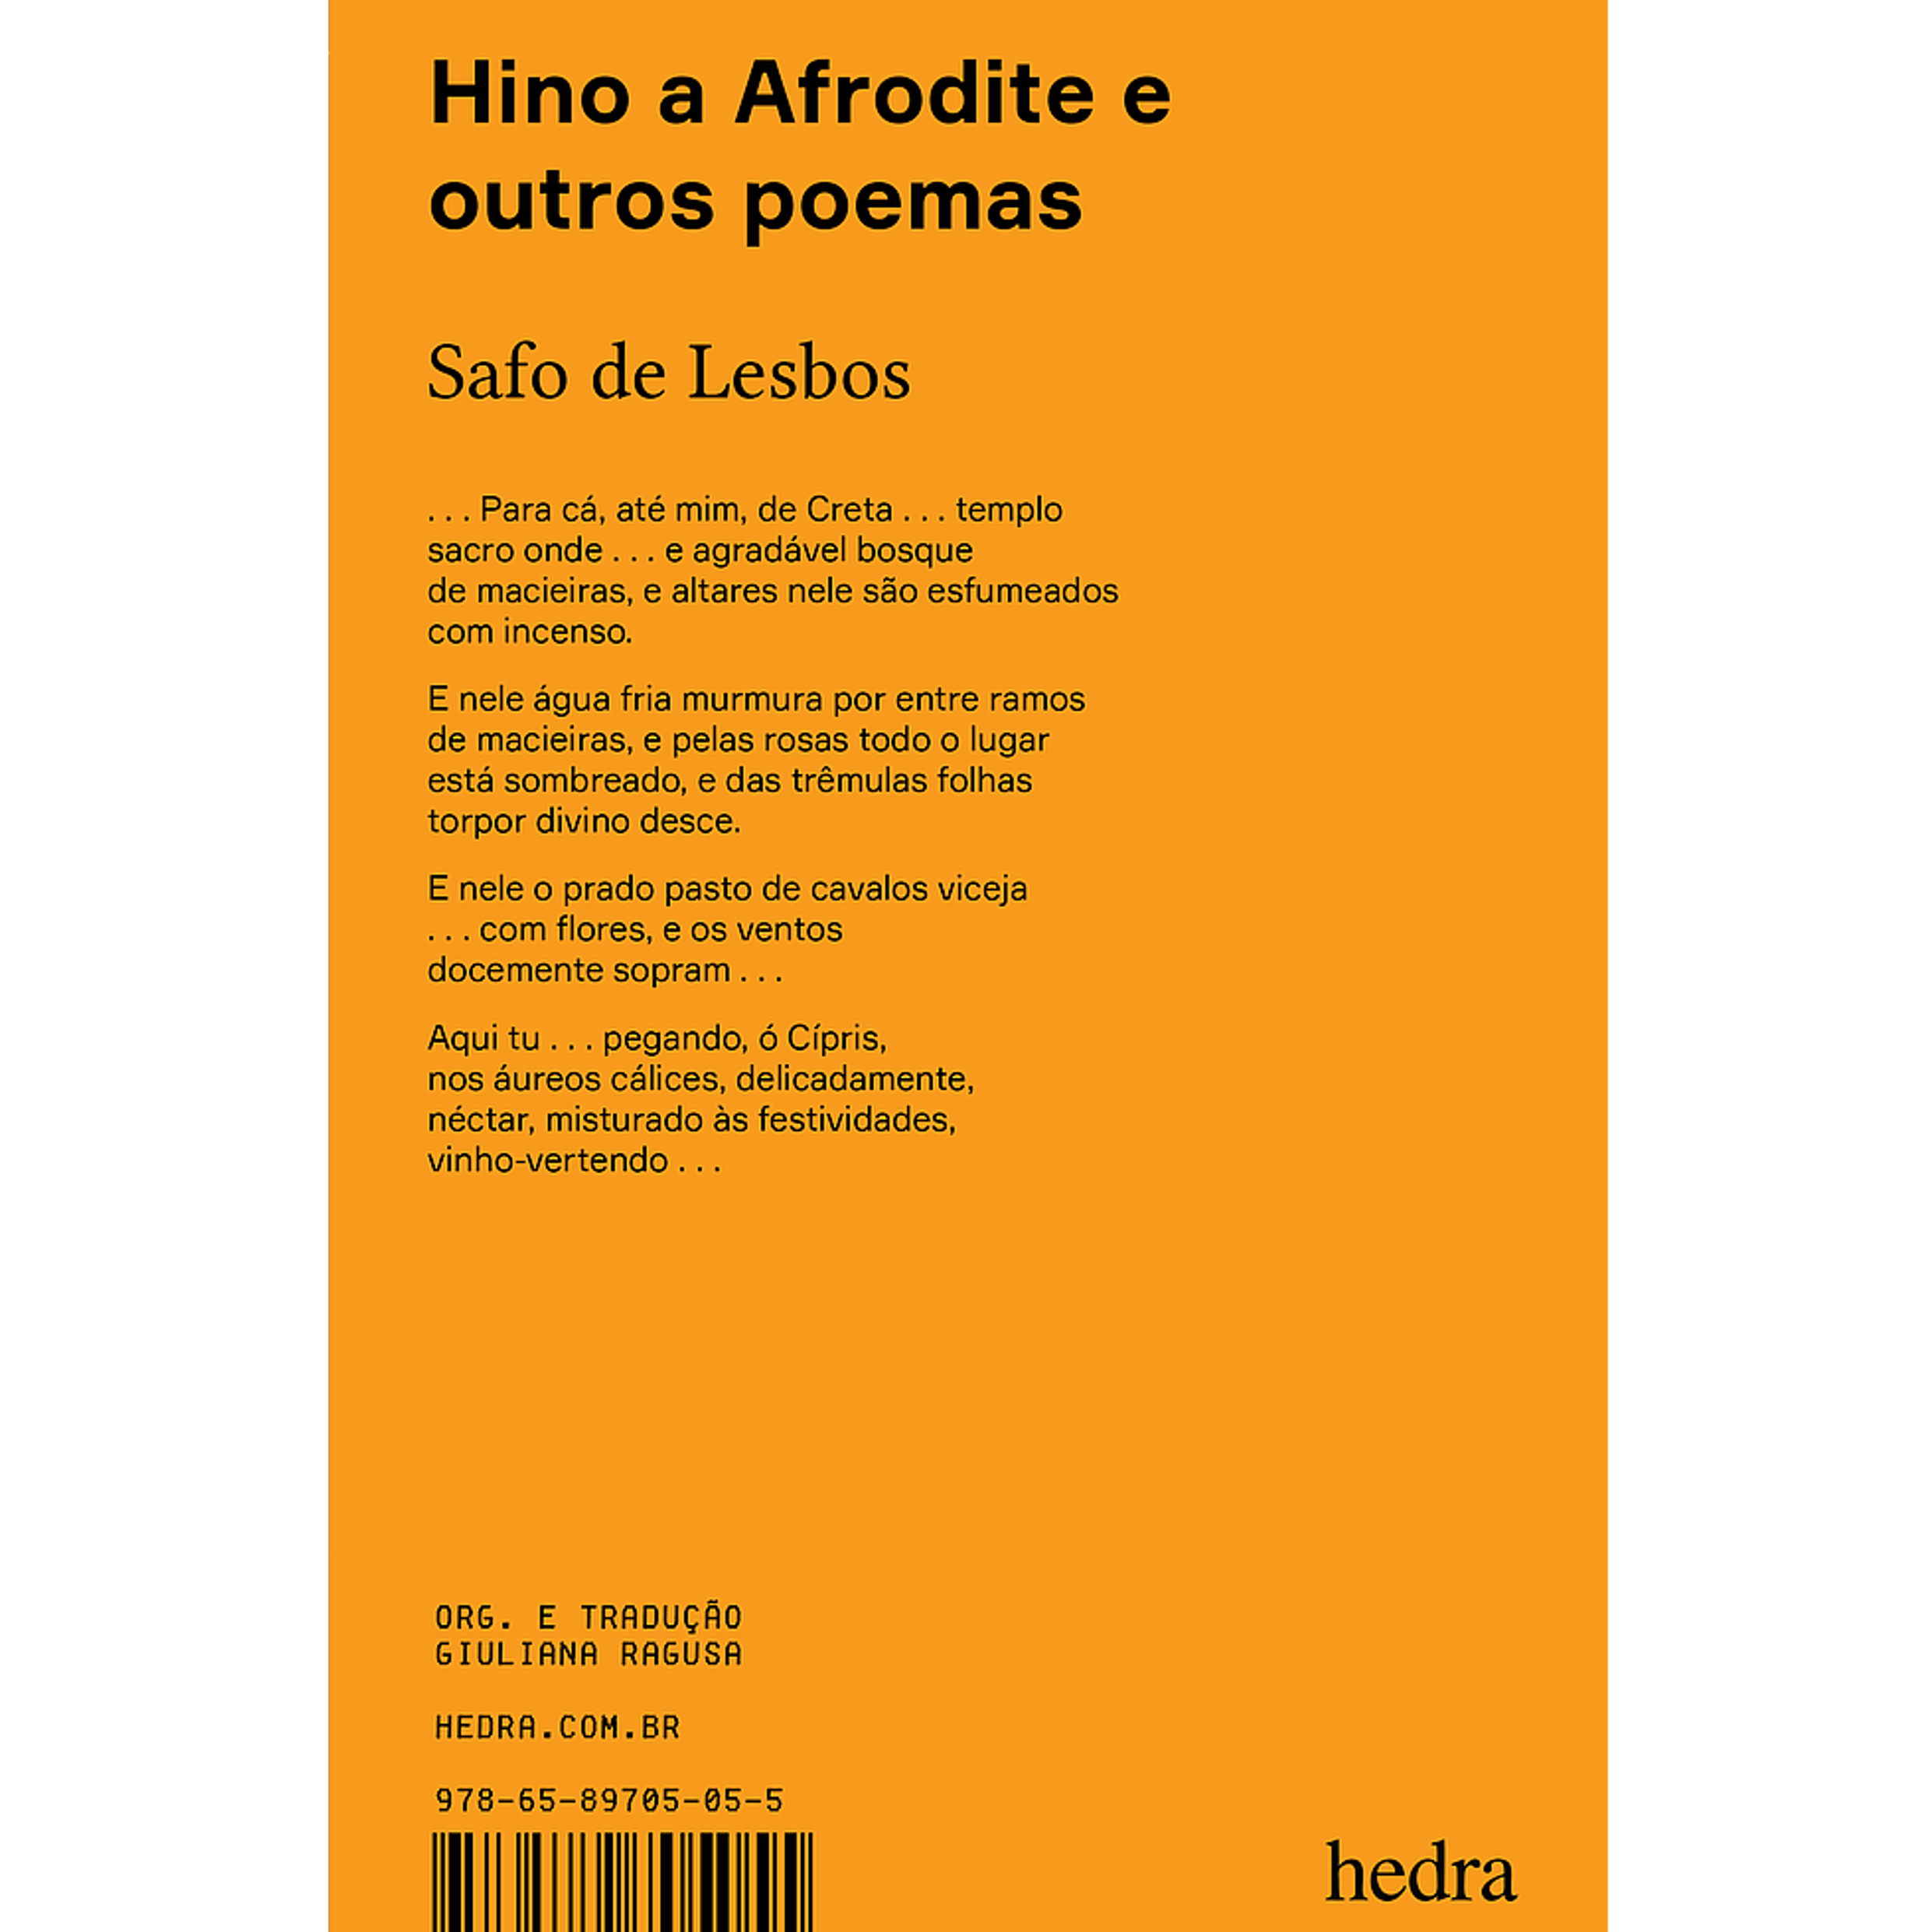
\includegraphics[width=74mm]{./CAPAS/HEDRA_SAFO.jpg}
% \end{center}
% \hspace*{-7cm}\hrulefill\hspace*{-7cm}
% \medskip

% \noindent{}Reunião de \hlc{textos remanescentes da mélica de Safo, ou seja, as canções para performance ao som da lira. Os textos aqui são traduzidos e anotados por Giuliana Ragusa em segunda edição --- com novos poemas, atualizações e em versão bilíngue} ---, autora que ganhou o Jabuti 2006 com um livro sobre a lírica da poeta, a única mulher entre os grandes da época. Para esta edição foram selecionados a única canção completa e os fragmentos mais legíveis de canções do corpus de Safo. As anotações de leitura buscam lançar luz sobre elementos relevantes da estrutura, conteúdo ou transmissão dos fragmentos organizados tematicamente. Precede a tradução anotada uma introdução sobre a poeta, sua poesia e o contexto em que se produziu e circulou, o gênero mélico, a fortuna crítica sobre ela, a transmissão de sua obra, e as outras poetas mulheres de que se tem notícia.

% \vfill
% \noindent\begin{minipage}[c]{1\linewidth}
% {\small\textbf{
% \hspace*{-.1cm}Editora: Hedra\\
% Título: Hino a Afrodite e outros poemas\\
% Autor: Safo de Lesbos\\ 
% ISBN: 978-65-89705-05-5\\
% Páginas: 212\\
% Formato: 13,3x21\,cm\\
% Preço: R\$ 69,00\\
% }}
% \end{minipage}
% \pagebreak

% \begin{center}
% \hspace*{.5cm}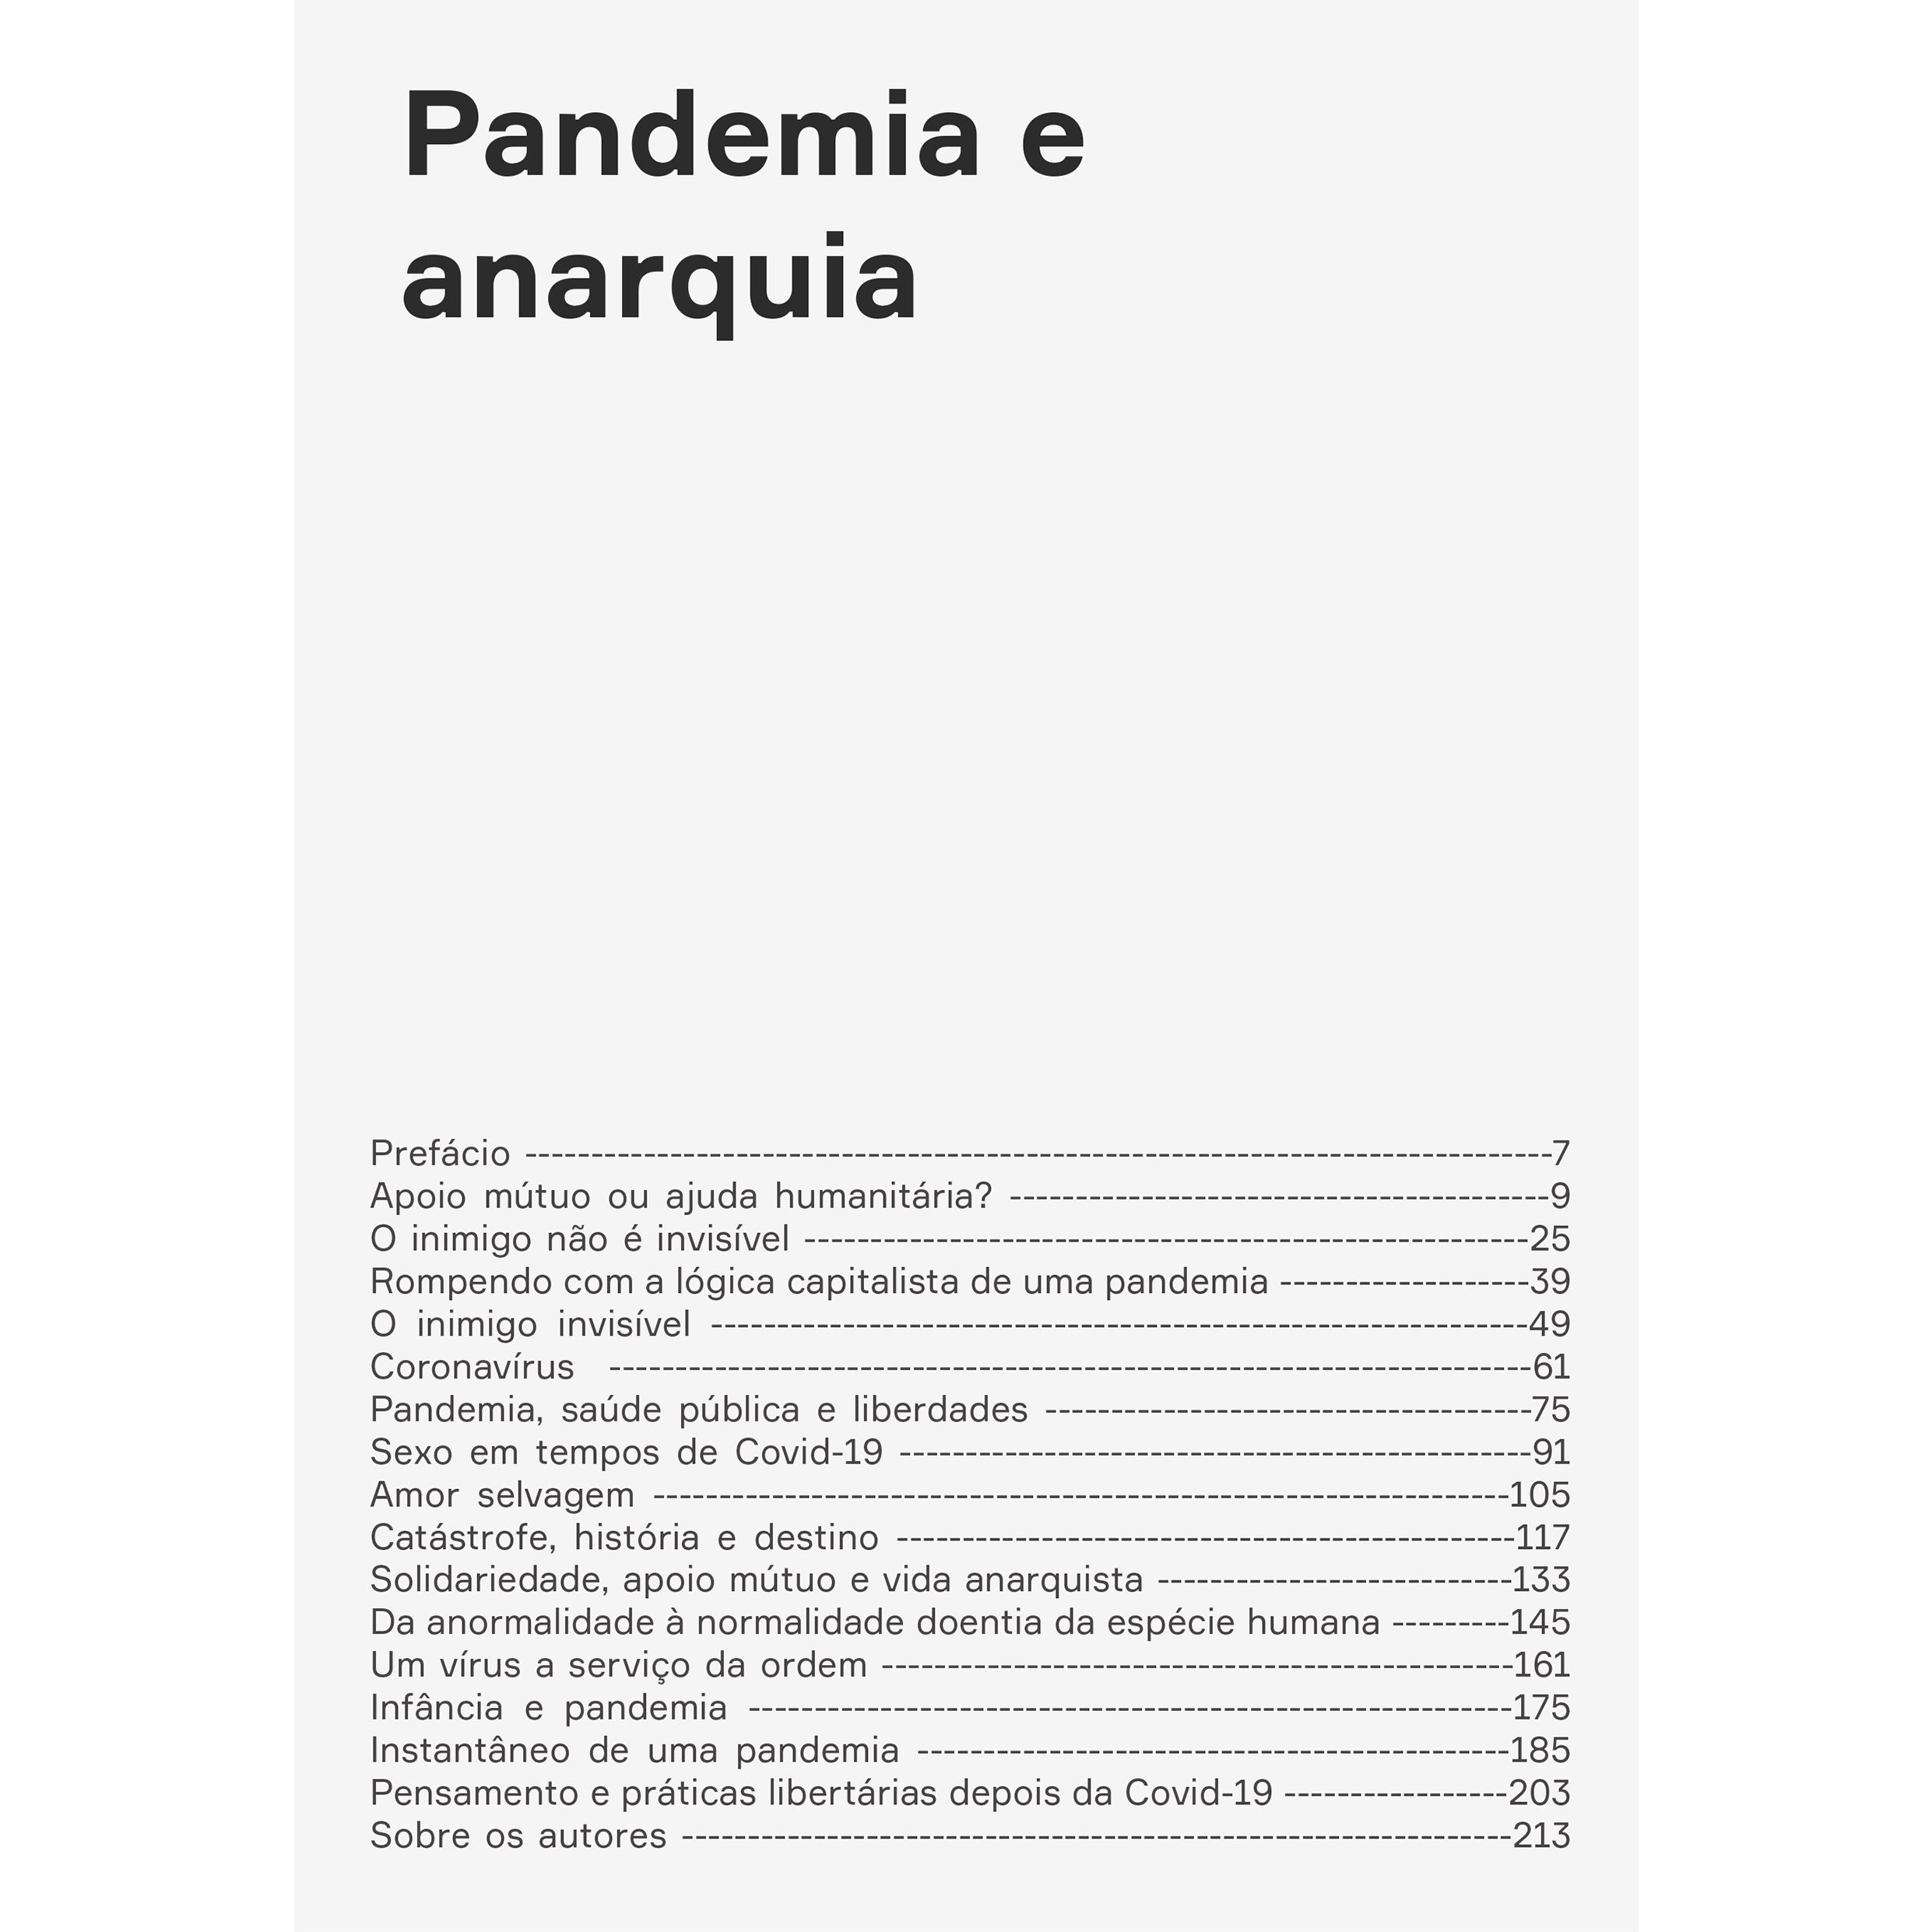
\includegraphics[width=74mm]{./CAPAS/HEDRA_PANDEMIA.jpg}
% \end{center}
% \hspace*{-7cm}\hrulefill\hspace*{-7cm}
% \medskip

% \noindent{}\textit{Pandemia e anarquia} reúne quinze ensaios de pesquisadores das práticas libertárias que analisam as implicações sociopolíticas do novo coronavírus e sua relação com os modos de existência. Além da Somaterapia e de pesquisadores do Nu-Sol (Núcleo de Sociabilidade Libertária), este livro traz escritos de historiadores e cientistas políticos residentes em diversos espaços do planeta. Perpassando diversas esferas das relações humanas, da economia e da ciência às relações amorosas e ao ser criança durante a pandemia, \hlc{os escritos insurgem-se contra a suposta ruptura com o mundo dado antes da Covid-19 para analisar e estancar a racionalidade neoliberal}, e a chamada crise sanitária. Com isso, traçam a afirmação de uma vida outra no presente.

% \vfill
% \noindent\begin{minipage}[c]{.5\linewidth}
% {\small\textbf{
% \hspace*{-.1cm}Editora: Hedra\\
% Título: Pandemia e anarquia\\
% Autor: Edson Passetti, João da Mata e José Maria Carvalho Ferreira (orgs.)\\ 
% ISBN: 978-65-89705-04-8\\
% Páginas: 220\\
% Formato: 16x23\,cm\\
% Preço: R\$ 69,00\\
% }}
% \end{minipage}
% \pagebreak

% \begin{center}
% \hspace*{-3.6cm}\raisebox{5cm}{\rotatebox[origin=t]{90}{\huge\textbf{Lançamento}}}
% \hspace*{3.1cm}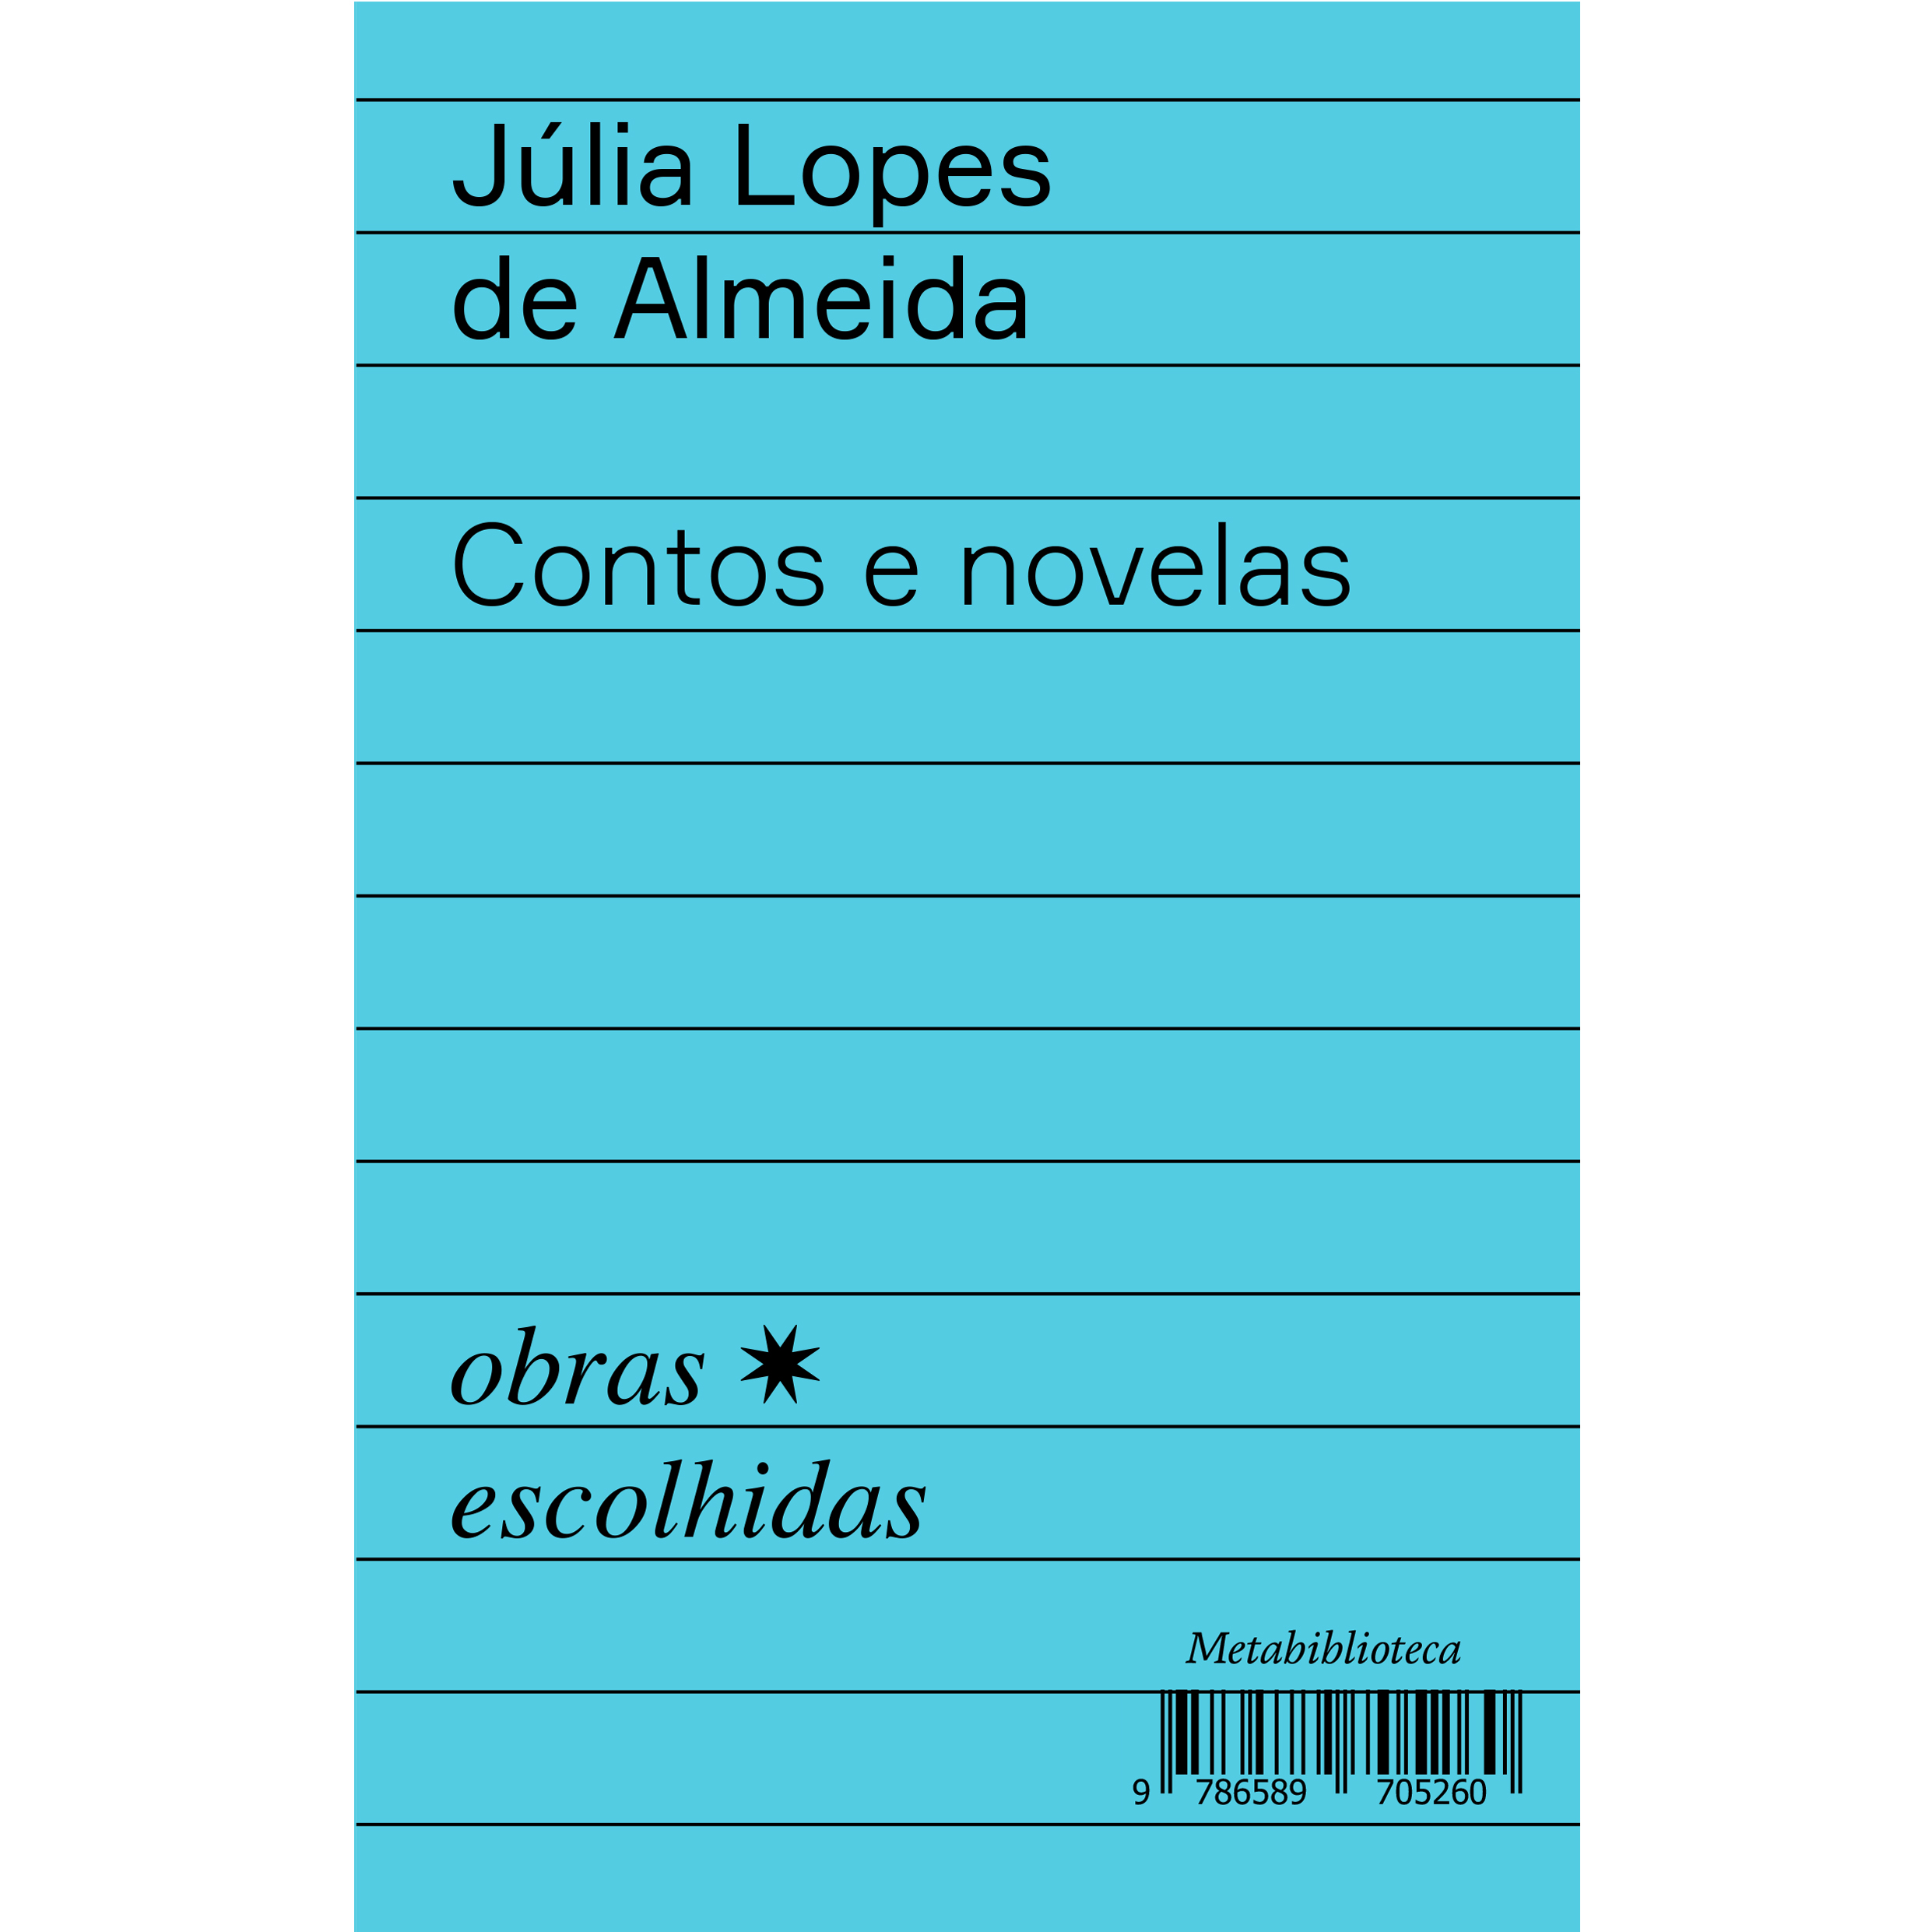
\includegraphics[width=74mm]{./CAPAS/HEDRA_JULIA.jpg}
% \end{center}
% \hspace*{-7cm}\hrulefill\hspace*{-7cm}
% \medskip

% \noindent{}\textit{Contos e novelas} reúne narrativas curtas de Júlia Lopes de Almeida, extraídas de duas de suas obras: \textit{Ânsia eterna} (1903) e \textit{A isca} (1922). Da primeira, fortemente influenciada pelo escritor francês Guy de Maupassant, foram selecionados dez contos, marcados pelo insólito e pelo fantástico. Da segunda, que reunia originalmente quatro novelas, foram selecionadas duas que apresentam algumas das características da narrativa de Júlia Lopes e dos temas que permeiam sua obra. Com tintas do naturalismo e do realismo francês, sua prosa tem traços da objetividade, do antropocentrismo e do cientificismo que fizeram escola no século XIX. \hlc{Não ficam de fora, no entanto, as críticas à sociedade brasileira: o lugar da mulher na sociedade patriarcal, os conflitos familiares, as marcas da escravidão e os contrastes sociais, políticos e econômicos} resultantes da modernização são temas recorrentes.

% \vfill
% \noindent\begin{minipage}[c]{1\linewidth}
% {\small\textbf{
% \hspace*{-.1cm}Editora: Hedra\\
% Título: Contos e novelas: obras escolhidas\\
% Autor: Júlia Lopes de Almeida\\ 
% ISBN: 978-65-89705-26-0\\
% Páginas: 190\\
% Formato: 13,3x21\,cm\\
% Preço: R\$ 64,00\\
% }}
% \end{minipage}
% \pagebreak

% \begin{center}
% \hspace*{.5cm}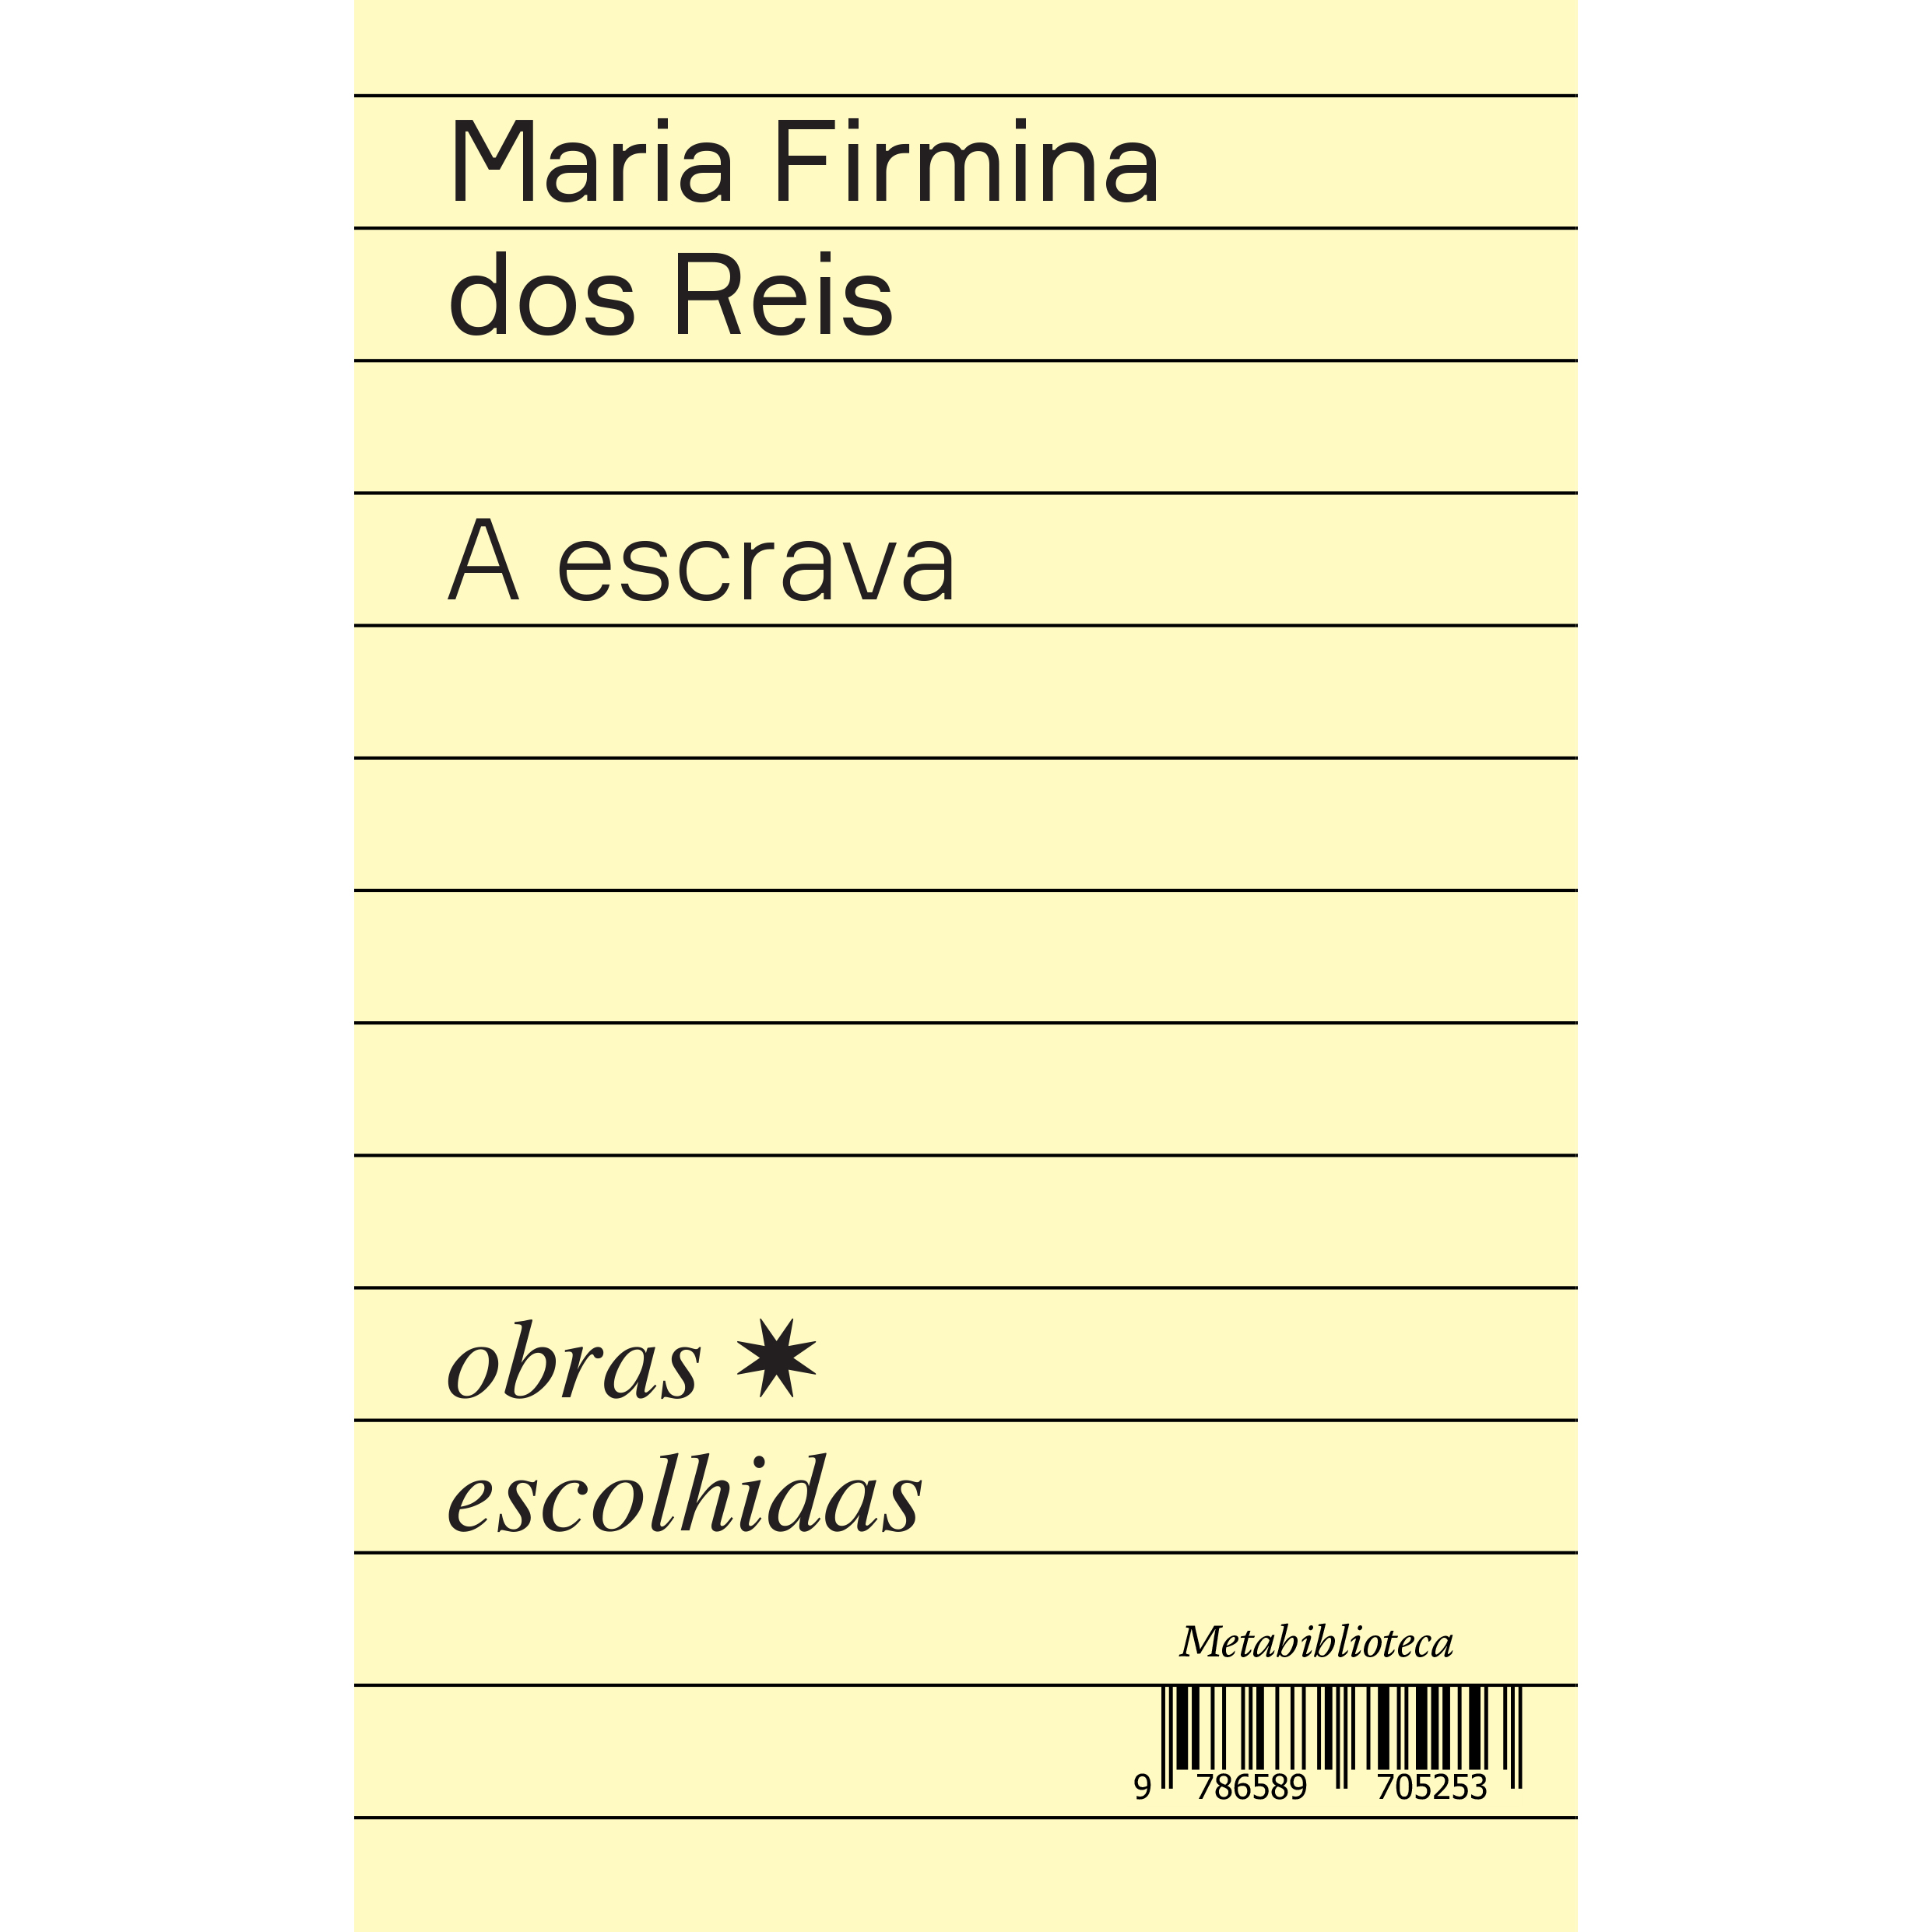
\includegraphics[width=74mm]{./CAPAS/HEDRA_FIRMINA.jpg}
% \end{center}
% \hspace*{-7cm}\hrulefill\hspace*{-7cm}
% \medskip

% \noindent{}\textit{A escrava} consiste em uma seleção de textos em prosa e poemas de Maria Firmina dos Reis (1822–1917), considerada a primeira romancista negra da história da literatura brasileira. Estão presentes o conto ``A escrava'', de 1887, a novela ``Gupeva'', de 1861, e 32 poemas: dos quais 29 foram extraídos entre os 56 de \textit{Cantos à beira-mar} (1871), dois da antologia \textit{Parnaso maranhense} (1861), e o famoso ``Hino à liberdade dos escravos'', originalmente escrito para ser cantado e acompanhado por instrumentos musicais. Nesta seleção, apresentam-se alguns dos principais elementos que caracterizam a literatura da escritora: \hlc{a situação dos escravizados, que passam a ter protagonismo nas narrativas, o papel da mulher na sociedade, as condições dos povos indígenas, um sentimentalismo romântico amoroso e a exaltação da terra.}

% \vfill
% \noindent\begin{minipage}[c]{1\linewidth}
% {\small\textbf{
% \hspace*{-.1cm}Editora: Hedra\\
% Título: A escrava: antologia de prosa e versos\\
% Autor: Maria Firmina dos Reis\\ 
% ISBN: 978-65-89705-25-3\\
% Páginas: 162\\
% Formato: 13,3x21\,cm\\
% Preço: R\$ 56,00\\
% }}
% \end{minipage}
% \pagebreak

\begin{center}
\hspace*{-3.6cm}\raisebox{5cm}{\rotatebox[origin=t]{90}{\huge\textbf{Lançamento}}}
\hspace*{3.1cm}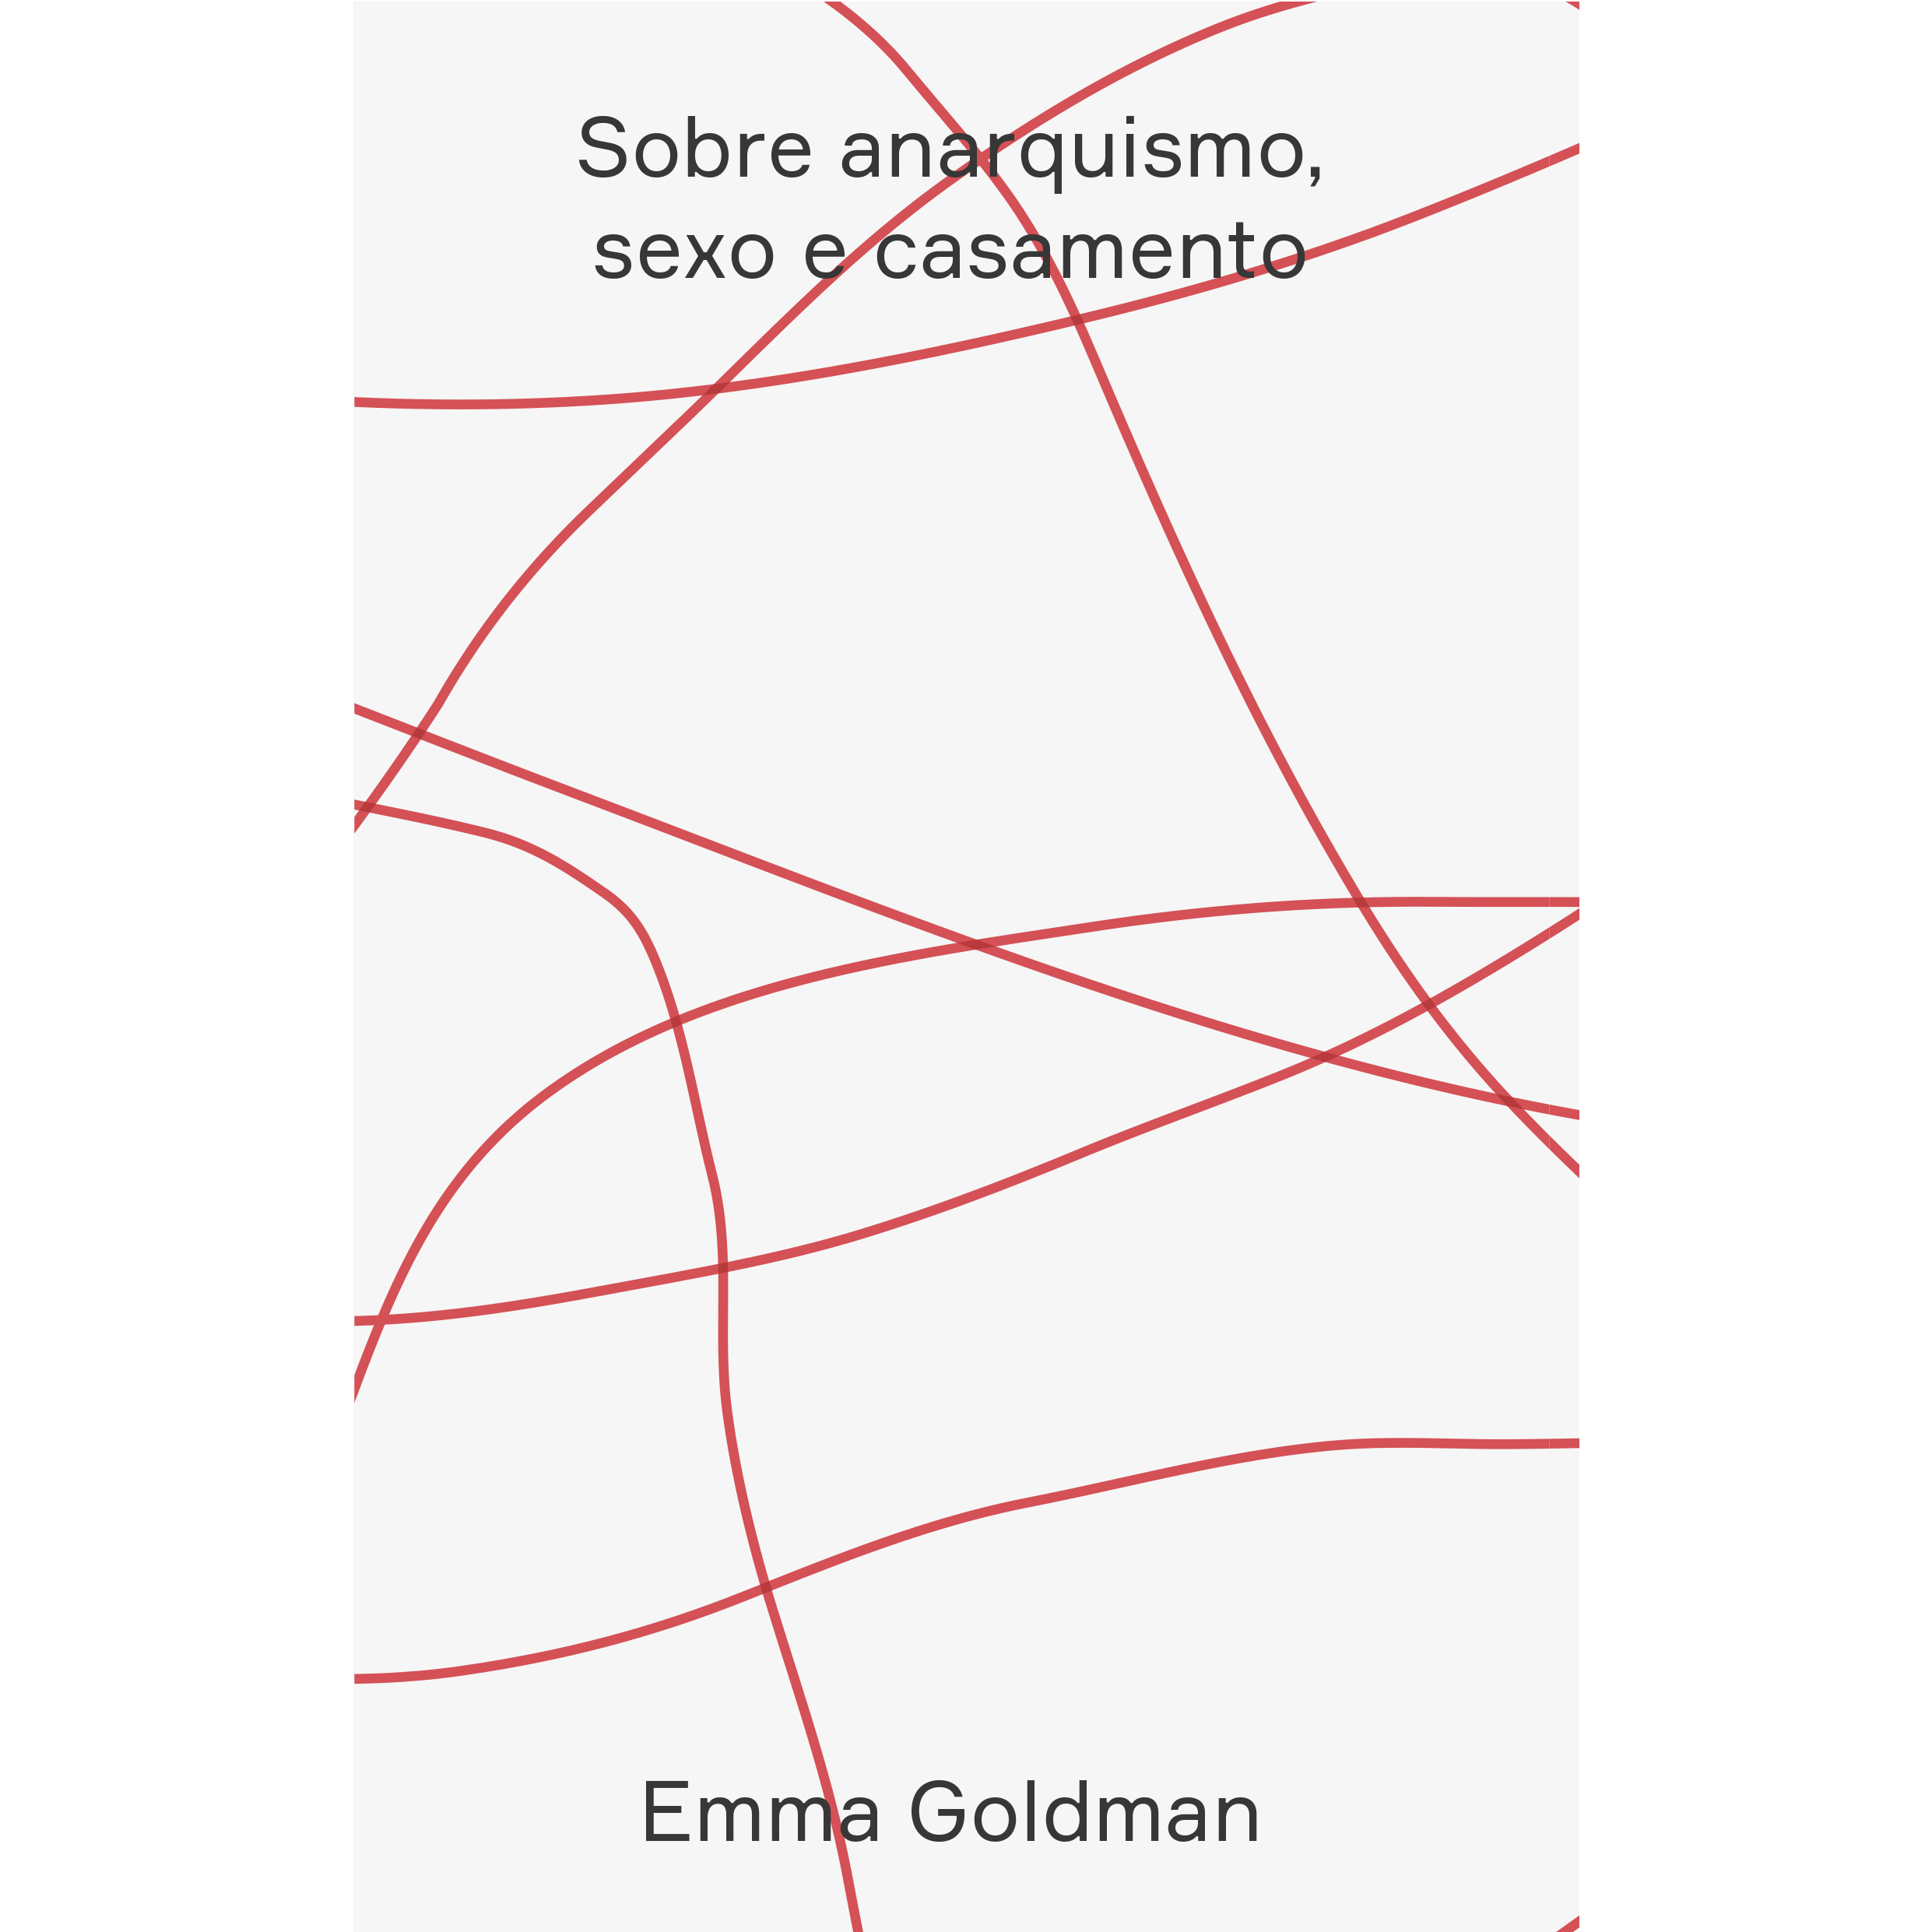
\includegraphics[width=74mm]{./CAPAS/HEDRA_GOLDMAN.jpg}
\end{center}
\hspace*{-7cm}\hrulefill\hspace*{-7cm}
\medskip

\noindent{}Sob perspectiva da implacável anarquista que foi Emma Goldman, \textit{Sobre anarquismo, sexo e casamento} trata de temas como o \hlc{controle de natalidade, o puritanismo norte-americano, a repressão sexual, o amor livre, o ciúme, a prostituição, a homossexualidade, a desigualdade entre os sexos, a maternidade, a emancipação feminina, o movimento sufragista na Inglaterra e Estados Unidos e a trajetória de uma série de mulheres extraordinárias}, dentre elas heroínas e mártires do movimento revolucionário russo. 

O contexto no qual esses textos foram escritos passou pela Primeira Guerra Mundial, a Revolução Russa e a ascensão do fascismo italiano e do nacional-socialismo na Alemanha. Dada a sua condição de russa, judia, anarquista e crítica implacável do puritanismo estadunidense à autocracia soviética, tornavam-lhe ainda mais vulnerável --- dos Estados Unidos à Rússia, e nos mais diferentes círculos.

\vfill
\noindent\begin{minipage}[c]{.5\linewidth}
{\small\textbf{
\hspace*{-.1cm}Editora: Hedra\\
Título: Sobre anarquismo,\\sexo e casamento\\
Autor: Emma Goldman\\ 
ISBN: 978-65-89705-23-9\\
Páginas: 264\\
Formato: 13,3x21\,cm\\
Preço: R\$ 77,90\\
}}
\end{minipage}
\pagebreak

\begin{center}
\hspace*{.5cm}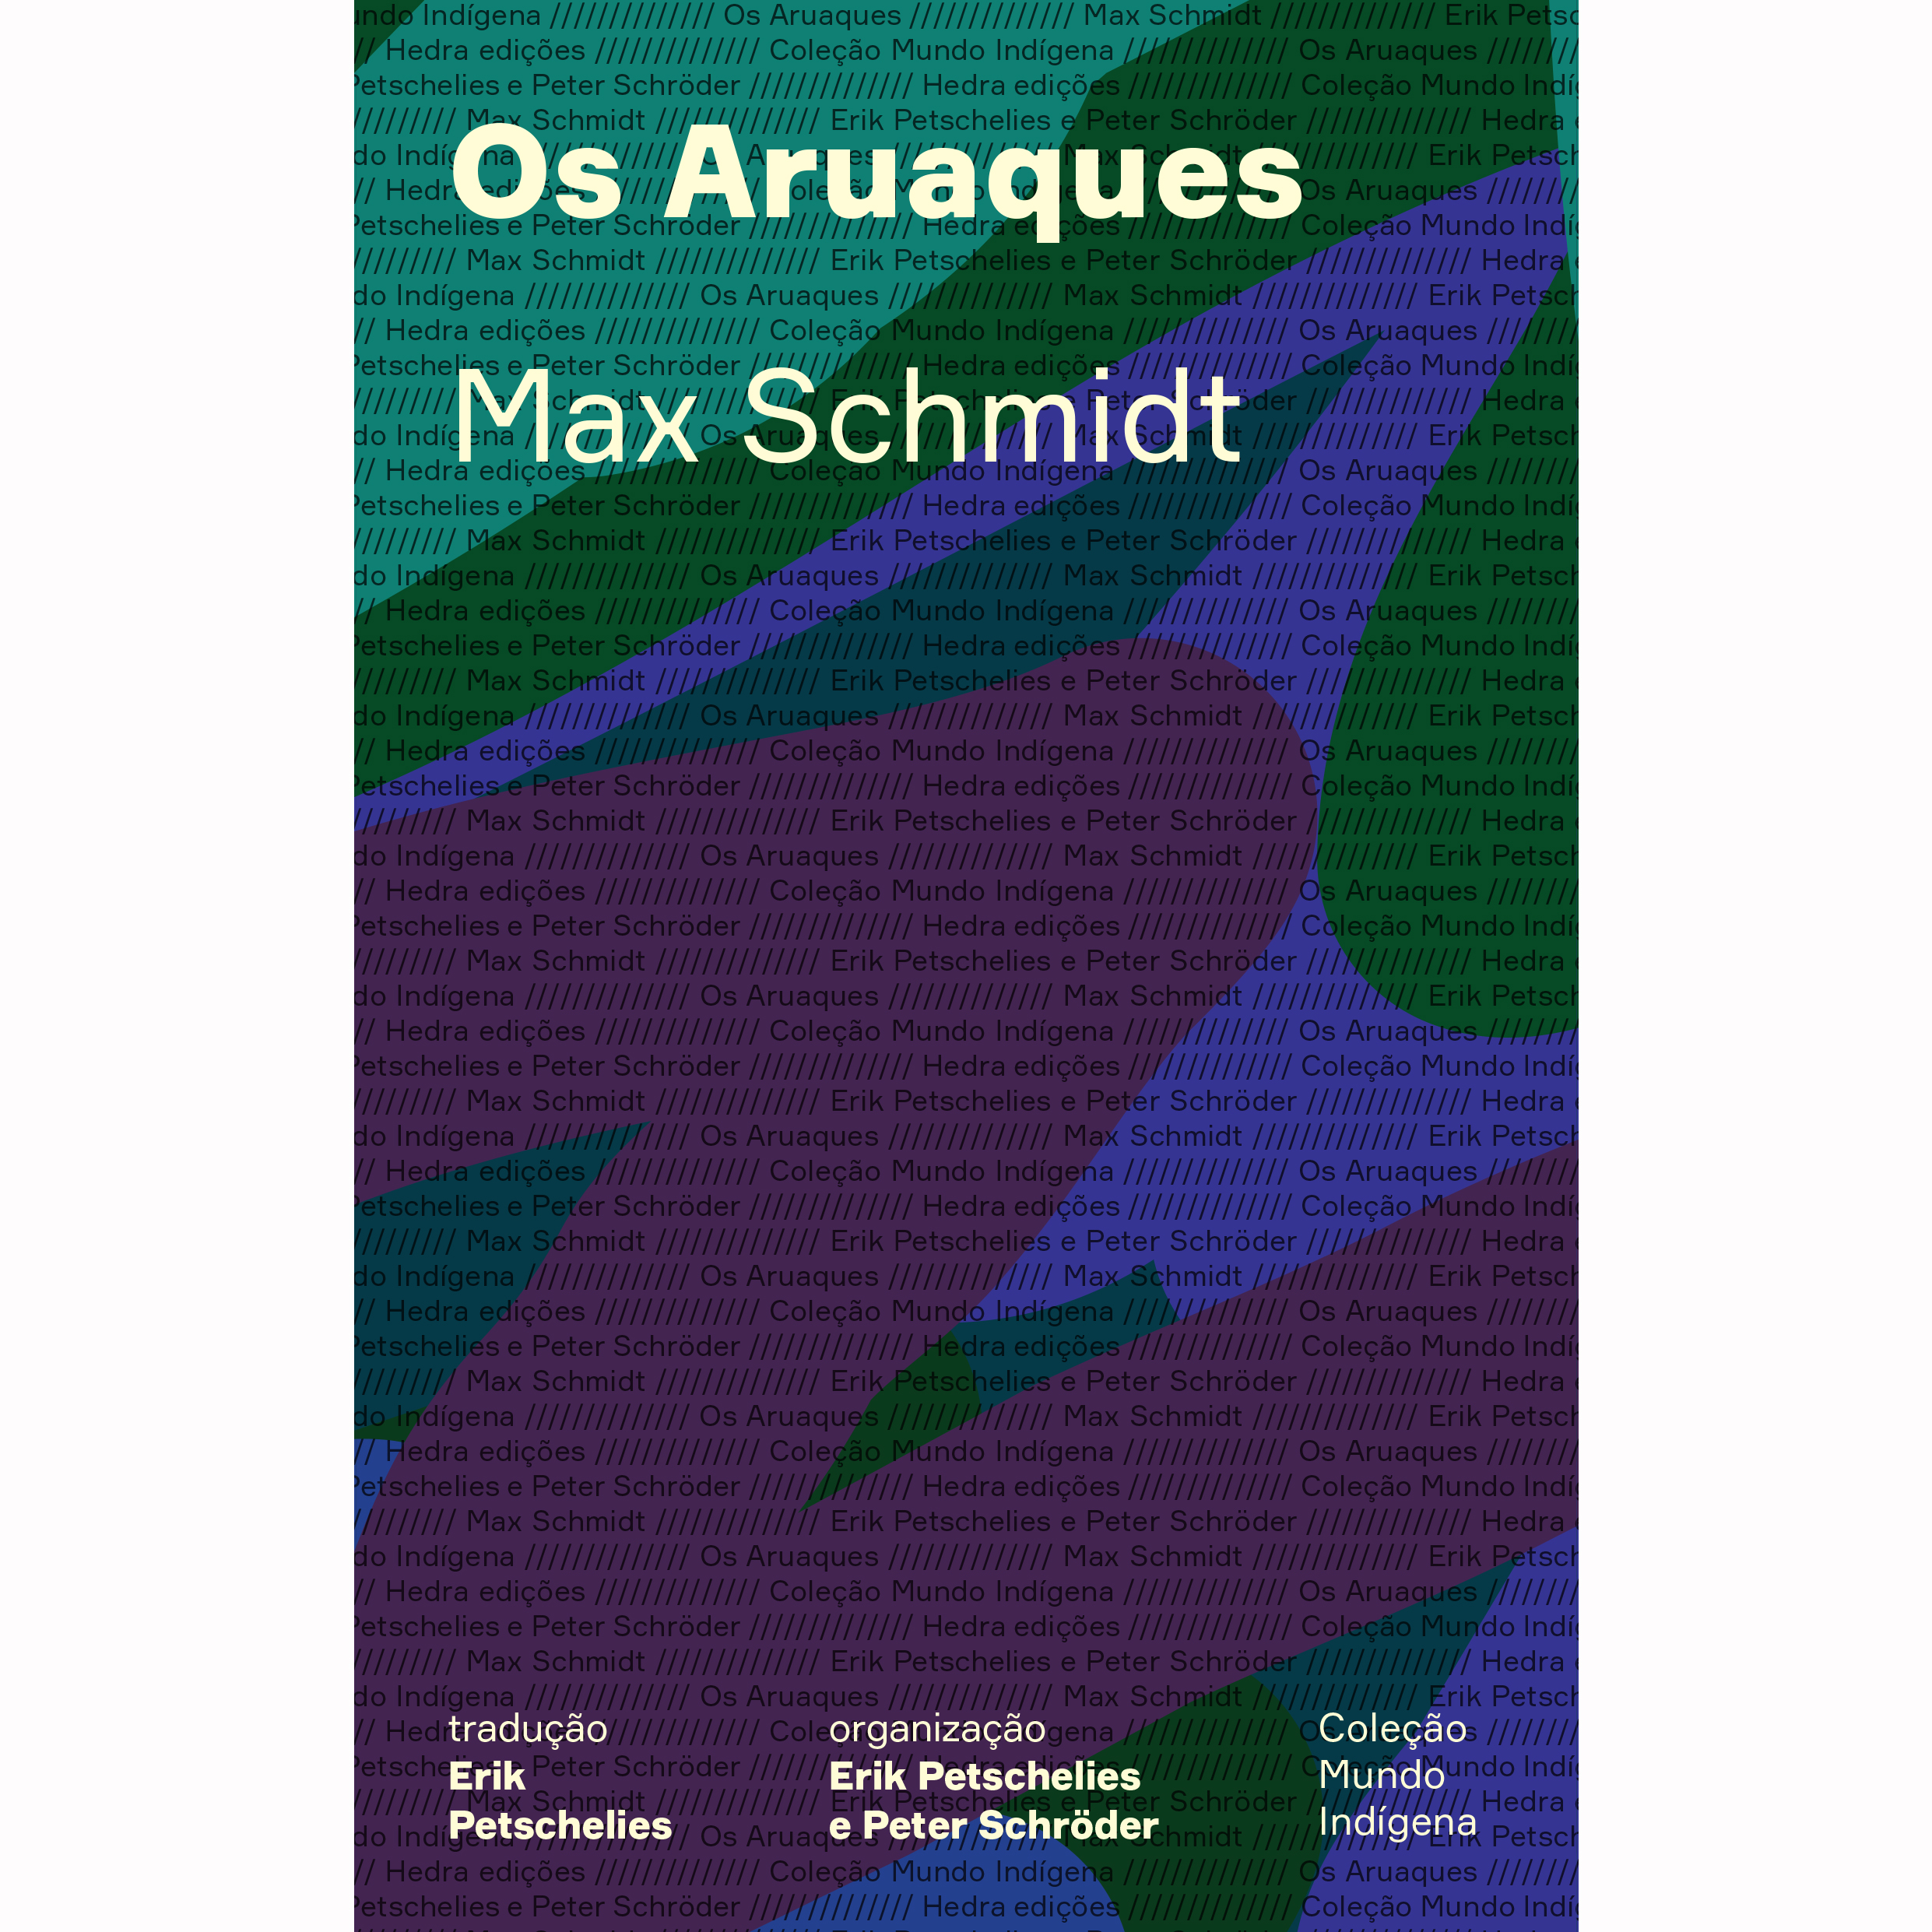
\includegraphics[width=74mm]{./CAPAS/HEDRA_ARUAQUES.jpg}
\end{center}
\hspace*{-7cm}\hrulefill\hspace*{-7cm}
\medskip

\noindent{}\textit{Os aruaques} é um \hlc{livro clássico, escrito antes da Primeira Guerra Mundial, sobre os povos indígenas falantes de línguas aruaque. Durante suas expedições, Max Schmidt já tinha observado a influência cultural dos povos aruaques sobre outros grupos, o que estimulou interesse por sua enorme expansão geográfica} nas terras baixas da América do Sul: o problema central não seria descobrir a origem geográfica dos aruaques, mas explicar sua dinâmica cultural. 

Schmidt opera com distinções claras entre língua e cultura, e conceitos como \textit{aculturação}, \textit{difusão} e \textit{mudança cultural}. Seu argumento principal é que outros autores, anteriores a ele, não teriam levantado as questões certas sobre sua expansão, por isso a falta de respostas satisfatórias. Sua teoria de fato é diferente dos antecessores, mostrando grande originalidade para a época. \textit{Die Aruaken} é a segunda tese de doutorado de Max Schmidt (1874--1950), que já tinha realizado três expedições na América do Sul, em 1900--01, 1910 e 1914.

\vfill
\noindent\begin{minipage}[c]{1\linewidth}
{\small\textbf{
\hspace*{-.1cm}Editora: Hedra\\
Título: Os Aruaques\\
Autor: Max Schmidt\\ 
ISBN: 978-65-89705-22-2\\
Páginas: 182\\
Formato: 13,3x21\,cm\\
Preço: R\$ 57,00\\
}}
\end{minipage}
\pagebreak

\begin{center}
\hspace*{-3.6cm}\raisebox{5cm}{\rotatebox[origin=t]{90}{\huge\textbf{Lançamento}}}
\hspace*{3.1cm}
\includegraphics[width=74mm]{./CAPAS/HEDRA_SOCIEDADE.jpg}
\end{center}
\hspace*{-7cm}\hrulefill\hspace*{-7cm}
\medskip

\noindent{}As relações sociais passaram a figurar cada vez mais em ambientes digitais, e se transformaram em elementos de controle e disputas. É o \hlc{chamado \textit{capitalismo informacional}, baseado na coleta, monitoramento e análise de dados pessoais. Se deveriam circular livremente em redes distribuídas globalmente, têm sido coletados constantemente e utilizados sem que saibamos como e por quê} e, em grande parte, fora de regulamentação. É neste cenário que as corporações têm se apropriado da tecnologia para se colocar à frente da concorrência, ao passo que governos as usam como dispositivos de controle sobre os cidadãos. Para compreender esse fenômeno, pesquisadores se propõem a analisar neste livro as tensões da sociedade de controle, se apoiando nas contribuições de Gilbert Simondon, Félix Guattari, Gilles Deleuze, Maurizio Lazzarato, Michel Foucault, Manuel Castells, Frank Pasquale, Shoshana Zuboff, entre outros.

\vfill
\noindent\begin{minipage}[c]{1\linewidth}
{\small\textbf{
\hspace*{-.1cm}Editora: Hedra\\
Título: A sociedade de controle: manipulação e\\modulação nas redes digitais\\
Autor: Joyce Souza, Rodolfo Avelino e\\Sérgio Amadeu da Silveira (orgs.)\\ 
ISBN: 978-65-89705-19-2\\
Páginas: 160\\
Formato: 12,7x19,1\,cm\\
Preço: R\$ 59,00\\
}}
\end{minipage}
\pagebreak

\begin{center}
\hspace*{.5cm}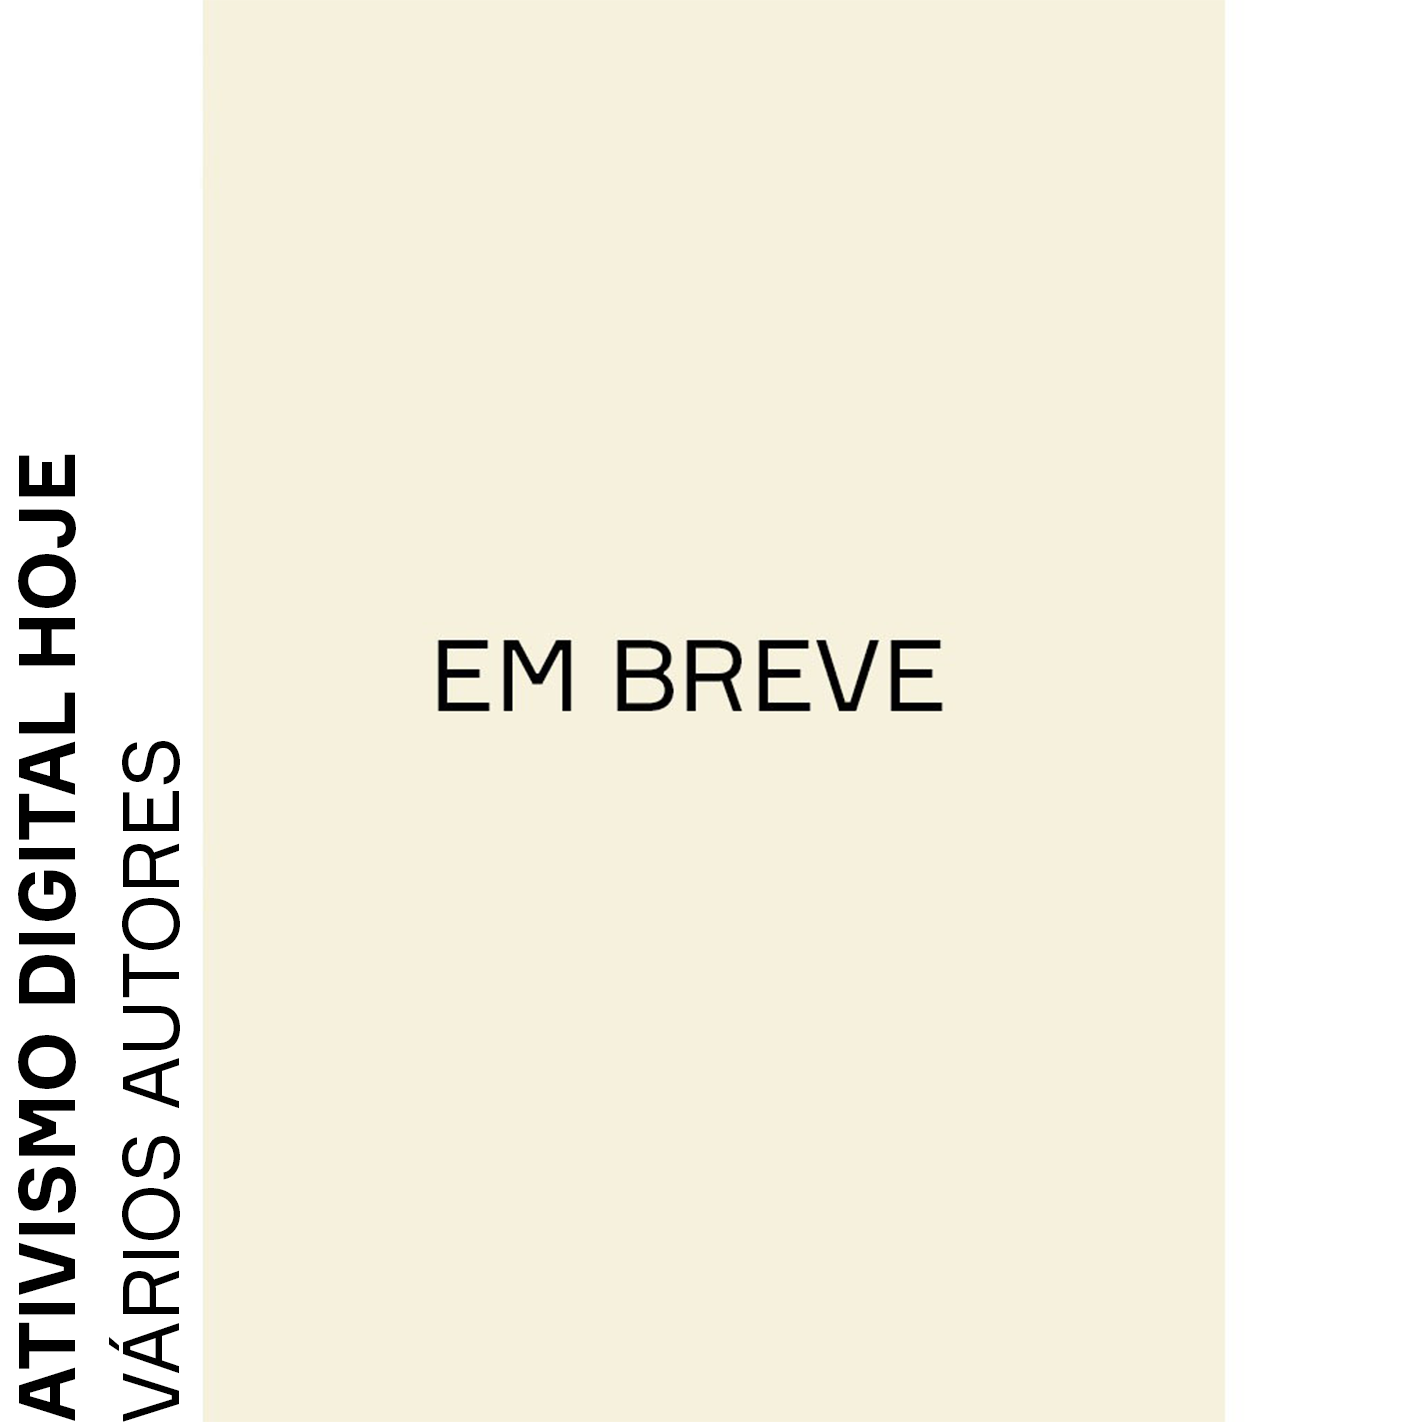
\includegraphics[width=74mm]{./CAPAS/HEDRA_ATIVISMO.jpg}
\end{center}
\hspace*{-7cm}\hrulefill\hspace*{-7cm}
\medskip

\noindent{}\textit{Ativismo digital hoje} reúne nove textos que refletem, de diferentes óticas, sobre a influência das redes sociais na política e na cultura atualmente: \hlc{ciberfeminismo, democracia digital, políticas online, ativismo online, cibervigilância, conflitos nas redes sociais, governo aberto, governança da Internet e cultura digital} são alguns dos temas explorados.
Pela abrangência do assunto, os artigos são divididos em três eixos: ciberpolítica, com enfoque na interface digital da política; ciberativismo, que percorre as alterações no campo do ativismo ocorridas desde a década de 1990; e cibercultura, que explora a emergência de práticas culturais e a expressão de subjetividades em consonância com as novas práticas comunicacionais do meio digital.

\vfill
\noindent\begin{minipage}[c]{1\linewidth}
{\small\textbf{
\hspace*{-.1cm}Editora: Hedra\\
Título: Ativismo digital hoje: política e\\cultura na era das redes\\
Autor: Rosemary Segurado, Claudio Penteado e\\Sérgio Amadeu da Silveira (orgs.)\\ 
ISBN: 978-85-7715-616-0\\
Páginas: 236\\
Formato: 12,7x19,1\,cm\\
Preço: R\$ 74,00\\
}}
\end{minipage}
\pagebreak

\begin{center}
\hspace*{-3.6cm}\raisebox{5cm}{\rotatebox[origin=t]{90}{\huge\textbf{Lançamento}}}
\hspace*{3.1cm}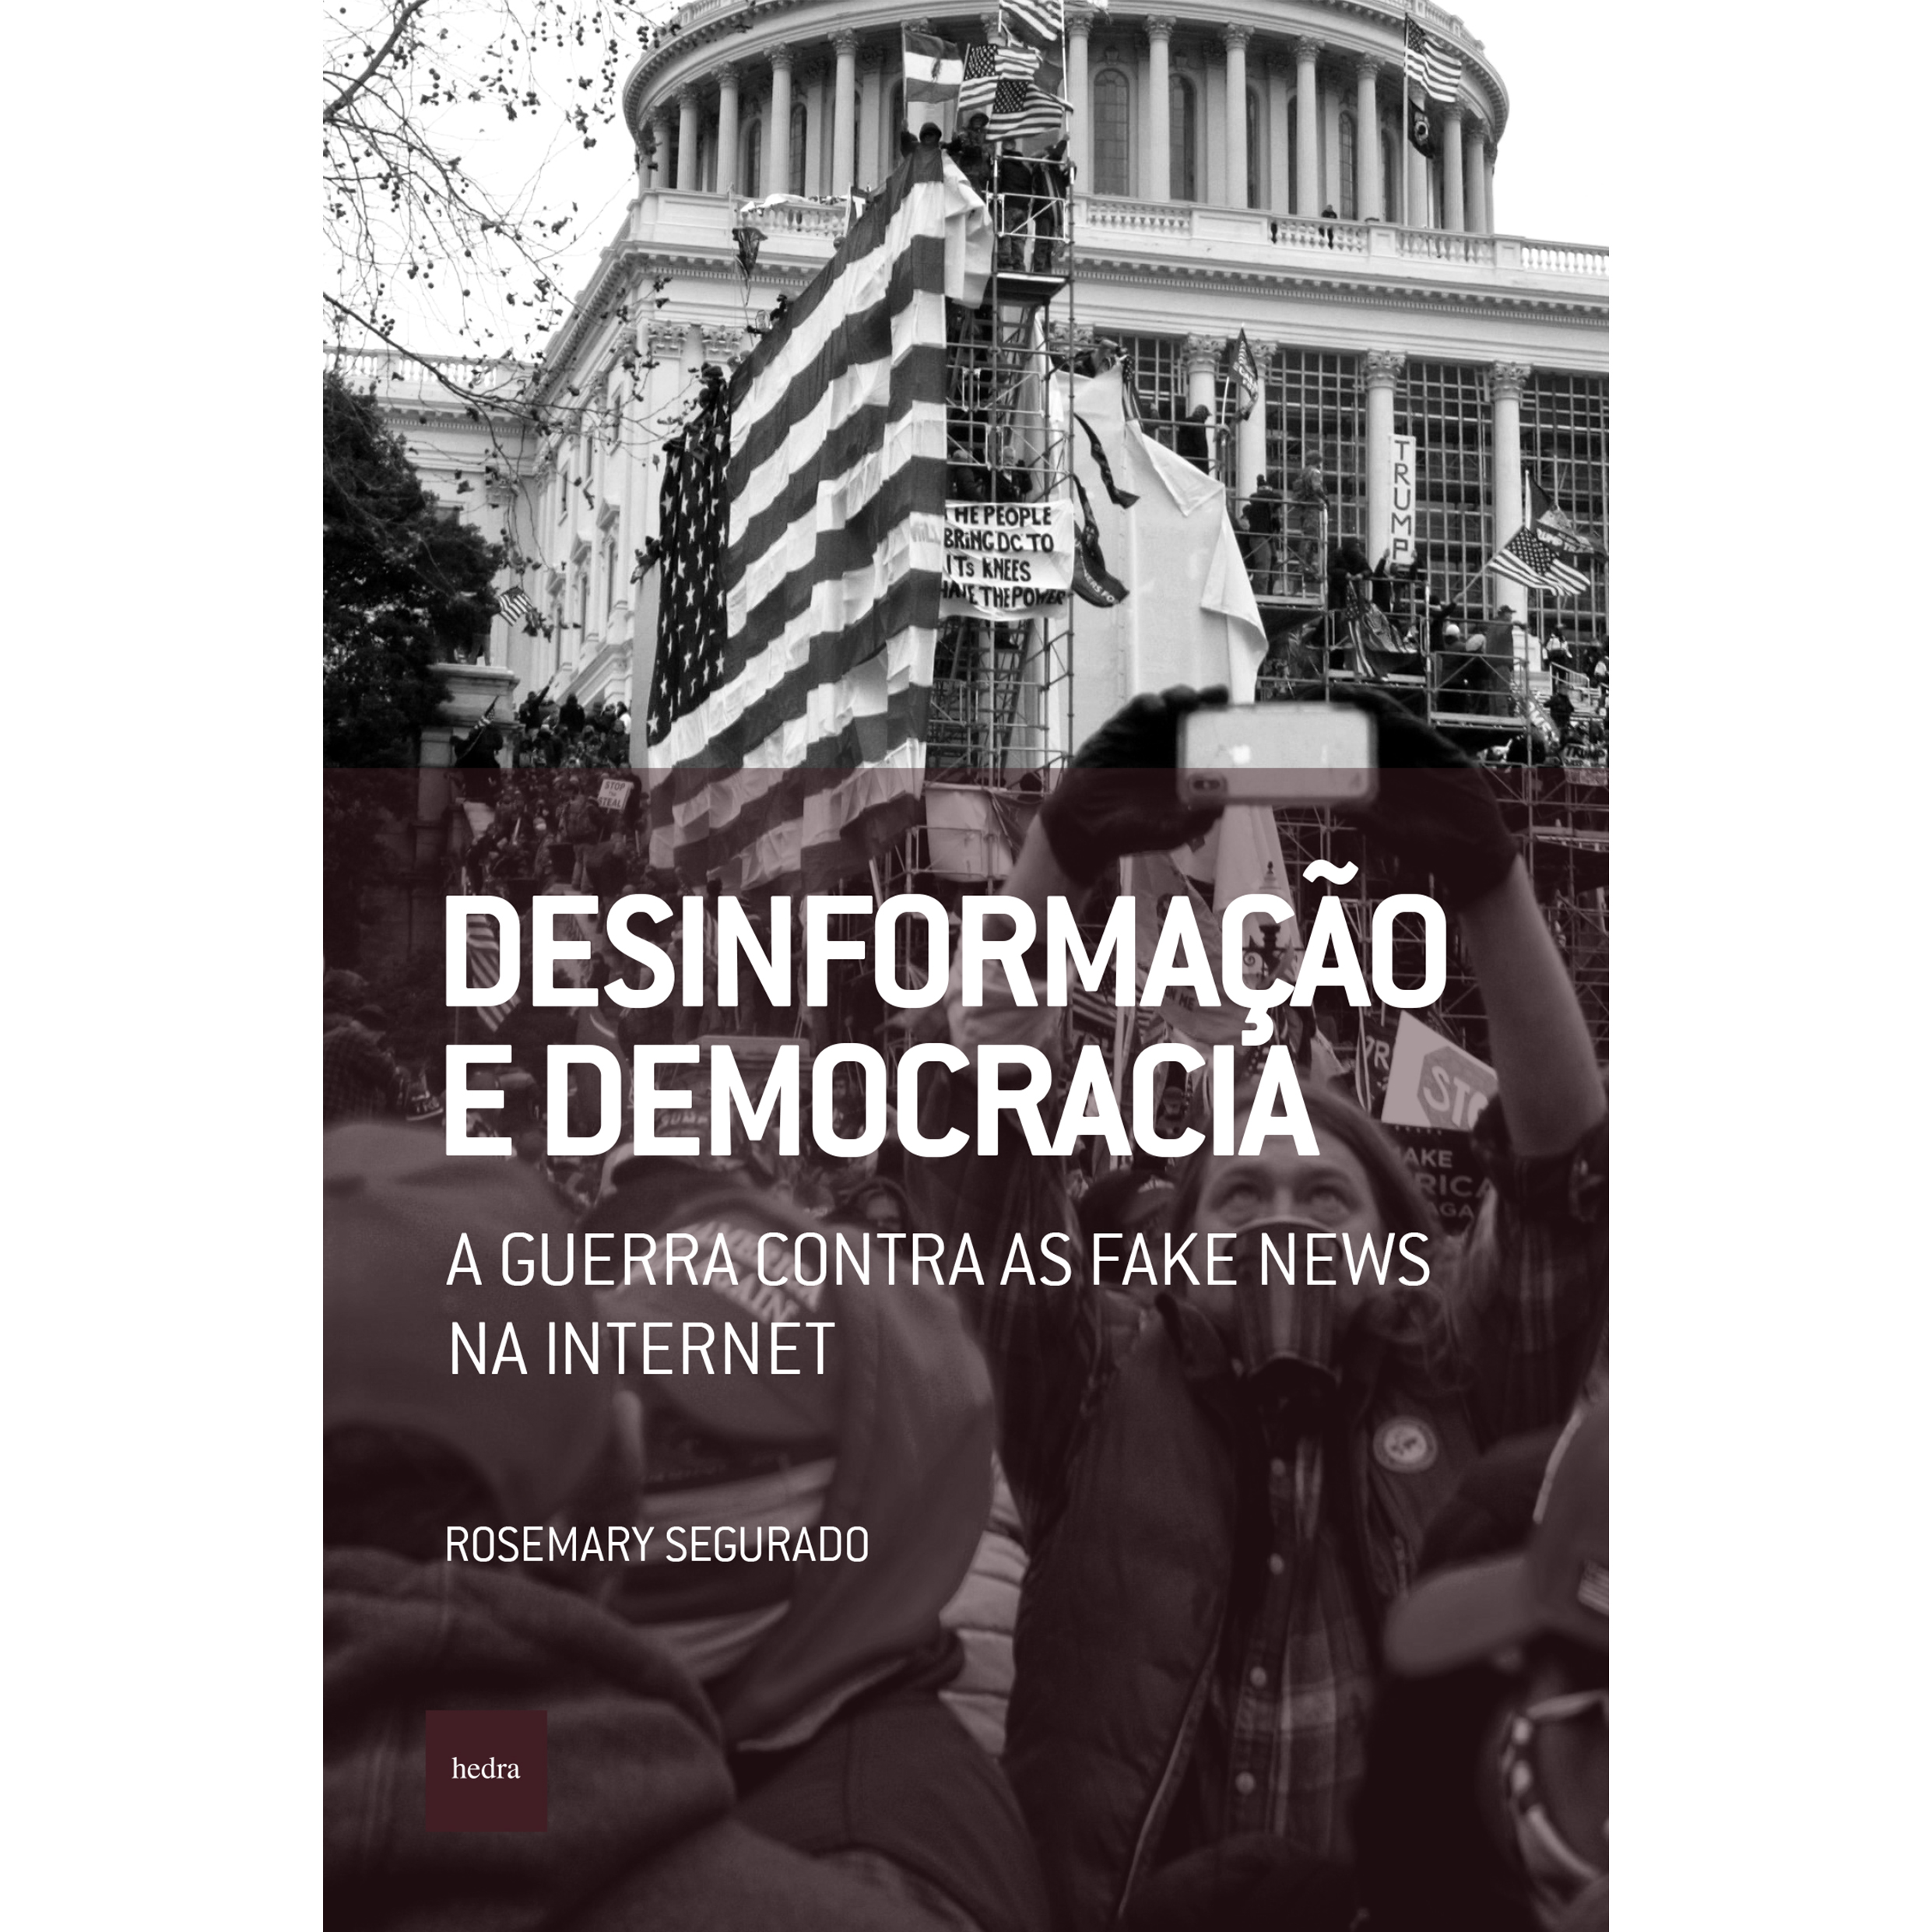
\includegraphics[width=74mm]{./CAPAS/HEDRA_DESINFORMACAO.jpg}
\end{center}
\hspace*{-7cm}\hrulefill\hspace*{-7cm}
\medskip

\noindent{}As plataformas digitais foram fundamentais para diminuir o impacto do distanciamento social durante a pandemia da Covid-19. A internet e as redes sociais digitais passaram a ser a janela para o mundo para muitos e através dela eram realizadas atividades profissionais, encontros entre amigos e familiares, compras e vendas online, aulas, consultas médicas e acesso à cultura. 

\hlc{A vida estava, enfim, circunscrita às telas de nossos computadores e celulares, embora a maior parte da população brasileira não pudesse se manter em isolamento social. Mas foi também por meio delas verificamos o aumento do compartilhamento de informações falsas}, mentiras e boatos sobre a pandemia. O Brasil ocupou o triste lugar de país que mais compartilha informações falsas ou duvidosas sobre o coronavírus.

\vfill
\noindent\begin{minipage}[c]{1\linewidth}
{\small\textbf{
\hspace*{-.1cm}Editora: Hedra\\
Título: Desinformação e democracia: a guerra contra as \textit{fake news} na internet\\
Autor: Rosemary Segurado (org.)\\
ISBN: 978-65-89705-34-5\\
Páginas: 130\\
Formato: 12,7x19,1\,cm\\
Preço: R\$ 52,90\\
}}
\end{minipage}
\pagebreak

\begin{center}
\hspace*{.5cm}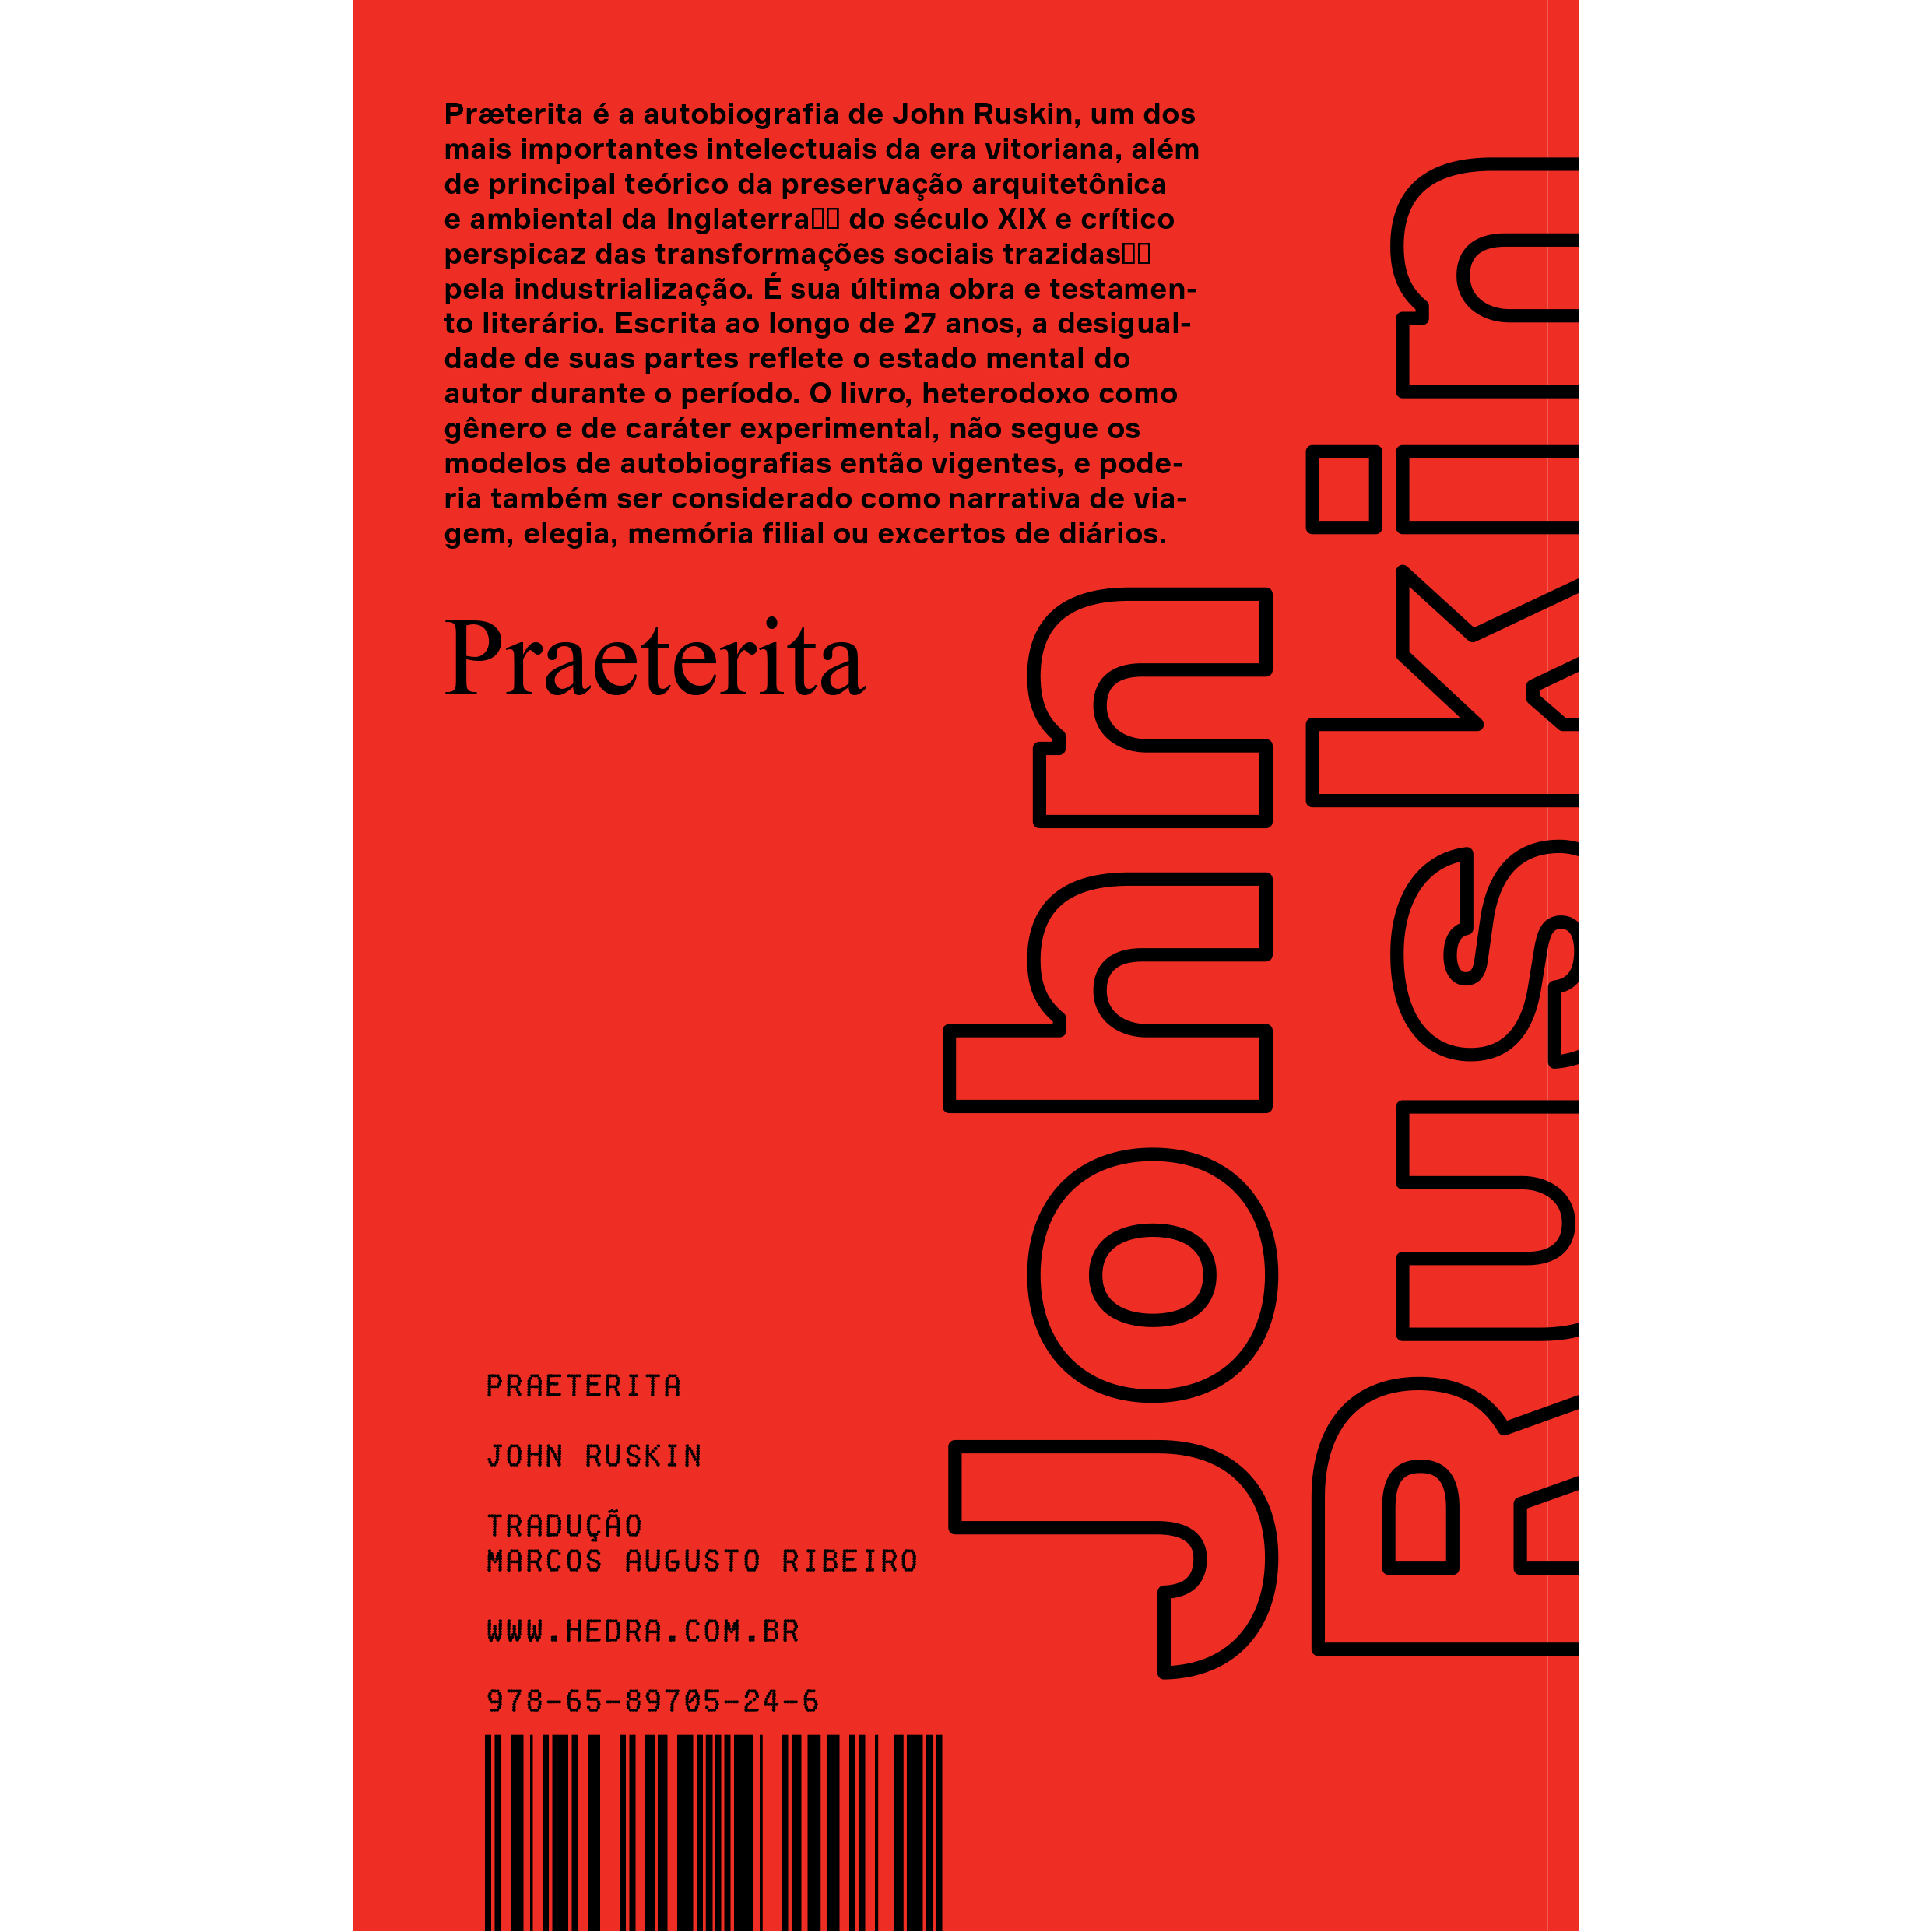
\includegraphics[width=74mm]{./CAPAS/HEDRA_RUSKIN.jpg}
\end{center}
\hspace*{-7cm}\hrulefill\hspace*{-7cm}
\medskip

\noindent{}John Ruskin (1819--1900), \hlc{foi um dos mais importantes intelectuais da era vitoriana. Principal teórico da preservação arquitetônica e ambiental da Inglaterra do século XIX e crítico perspicaz das transformações sociais trazidas ao país pela industrialização}, a qual veementemente combateu. Excêntrico, vinculado ao romantismo, grande esteta, valorizava a sensibilidade subjetiva em contraponto à razão; contraditório --- ao mesmo tempo aristocrático, reacionário e simpático ao socialismo. \textit{Pr\ae t\textls[-470]{e˘}\textls[80]rita}, sua autobiografia, foi sua última obra e testamento literário. Escrita ao longo de 27 anos, a desigualdade de suas partes reflete o estado mental do autor durante o período de sua elaboração. O livro, heterodoxo como gênero e de caráter ``experimental'', não segue os modelos de autobiografias então vigentes --- geralmente apresentados em termos de confissão religiosa ---, e poderia também ser considerado como narrativa de viagem, elegia, memória filial ou coleção de excertos de diários. Esta tradução contempla apenas o primeiro dos três volumes de \textit{Pr\ae t\textls[-470]{e˘}\textls[80]rita}.

\vfill
\noindent\begin{minipage}[c]{1\linewidth}
{\small\textbf{
\hspace*{-.1cm}Editora: Hedra\\
Título: {Pr\ae t\textls[-470]{e˘}\textls[80]rita}\\
Autor: John Ruskin\\ 
ISBN: 978-65-89705-24-6\\
Páginas: 246\\
Formato: 13,3x21\,cm\\
Preço: R\$ 66,00\\
}}
\end{minipage}
\pagebreak

\begin{center}
\hspace*{-3.6cm}\raisebox{5cm}{\rotatebox[origin=t]{90}{\huge\textbf{Lançamento}}}
\hspace*{3.1cm}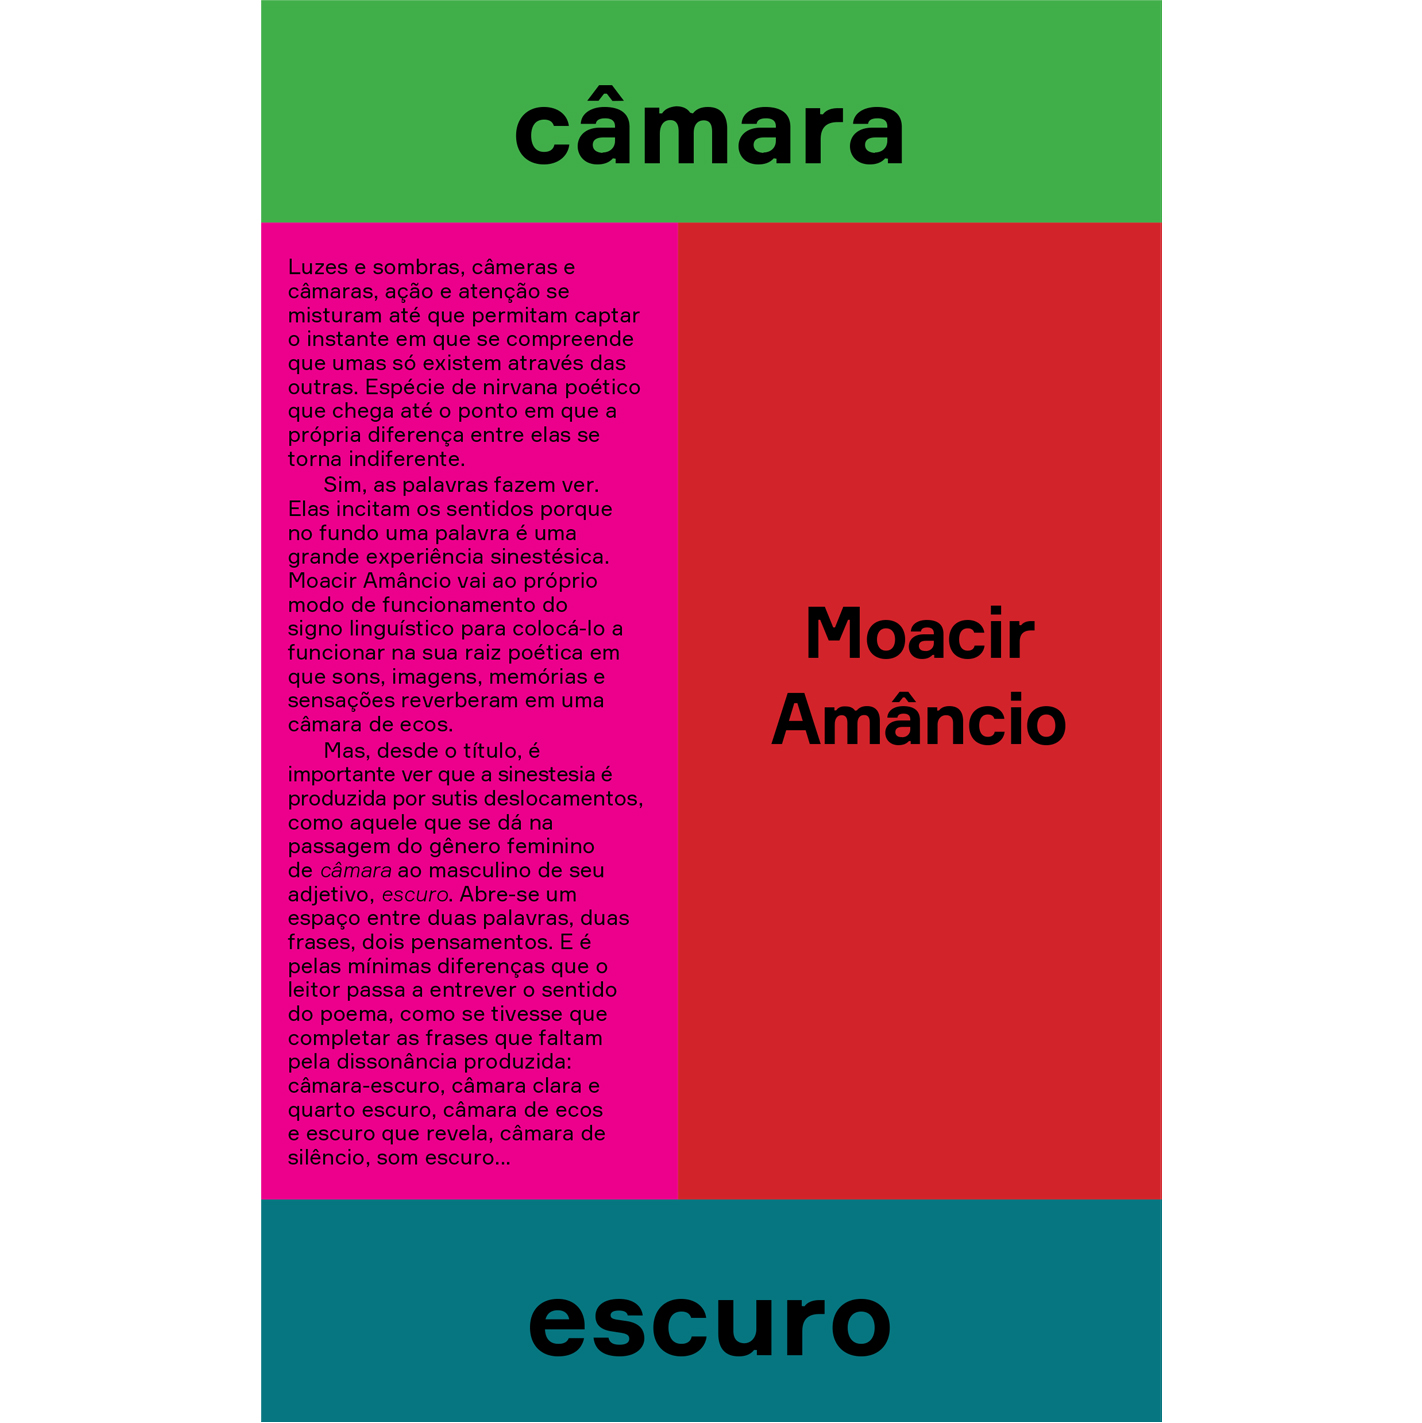
\includegraphics[width=74mm]{./CAPAS/HEDRA_CAMARA.jpg}
\end{center}
\hspace*{-7cm}\hrulefill\hspace*{-7cm}
\medskip

\noindent{}As palavras incitam os sentidos, pois são no fundo uma grande experiência sinestésica. \hlc{Moacir Amâncio vai ao próprio modo de funcionamento do signo linguístico para colocá-lo a funcionar na sua raiz poética em que sons, imagens, memórias e sensaçães reverberam em uma câmara de ecos.} Mas, desde o título, é importante ver que a sinestesia é produzida por sutis deslocamentos, como aquele que se dá na passagem do gênero feminino de \textit{câmara} ao masculino de seu adjetivo, \textit{escuro}. 

Abre-se um espaço entre duas palavras, duas frases, dois pensamentos. E é pelas mínimas diferenças que o leitor passa a entrever o sentido do poema, como se tivesse que completar as frases que faltam pela dissonância produzida: \textit{câmara-escuro}, \textit{câmara clara} e \textit{quarto escuro}, \textit{câmara de ecos} e \textit{escuro que revela}, \textit{câmara de silêncio}, \textit{som escuro}... Luzes e sombras, câmeras e câmaras, ação e atenção se misturam até que permitam captar o instante em que se compreende que umas só existem através das outras.

\vfill
\noindent\begin{minipage}[c]{1\linewidth}
{\small\textbf{
\hspace*{-.1cm}Editora: Hedra\\
Título: Câmara escuro\\
Autor: Moacir Amâncio\\ 
ISBN: 978-65-89705-27-7\\
Páginas: 78\\
Formato: 13,3x21\,cm\\
Preço: R\$ 35,90\\
}}
\end{minipage}
\pagebreak

% \begin{center}
% \hspace*{.5cm}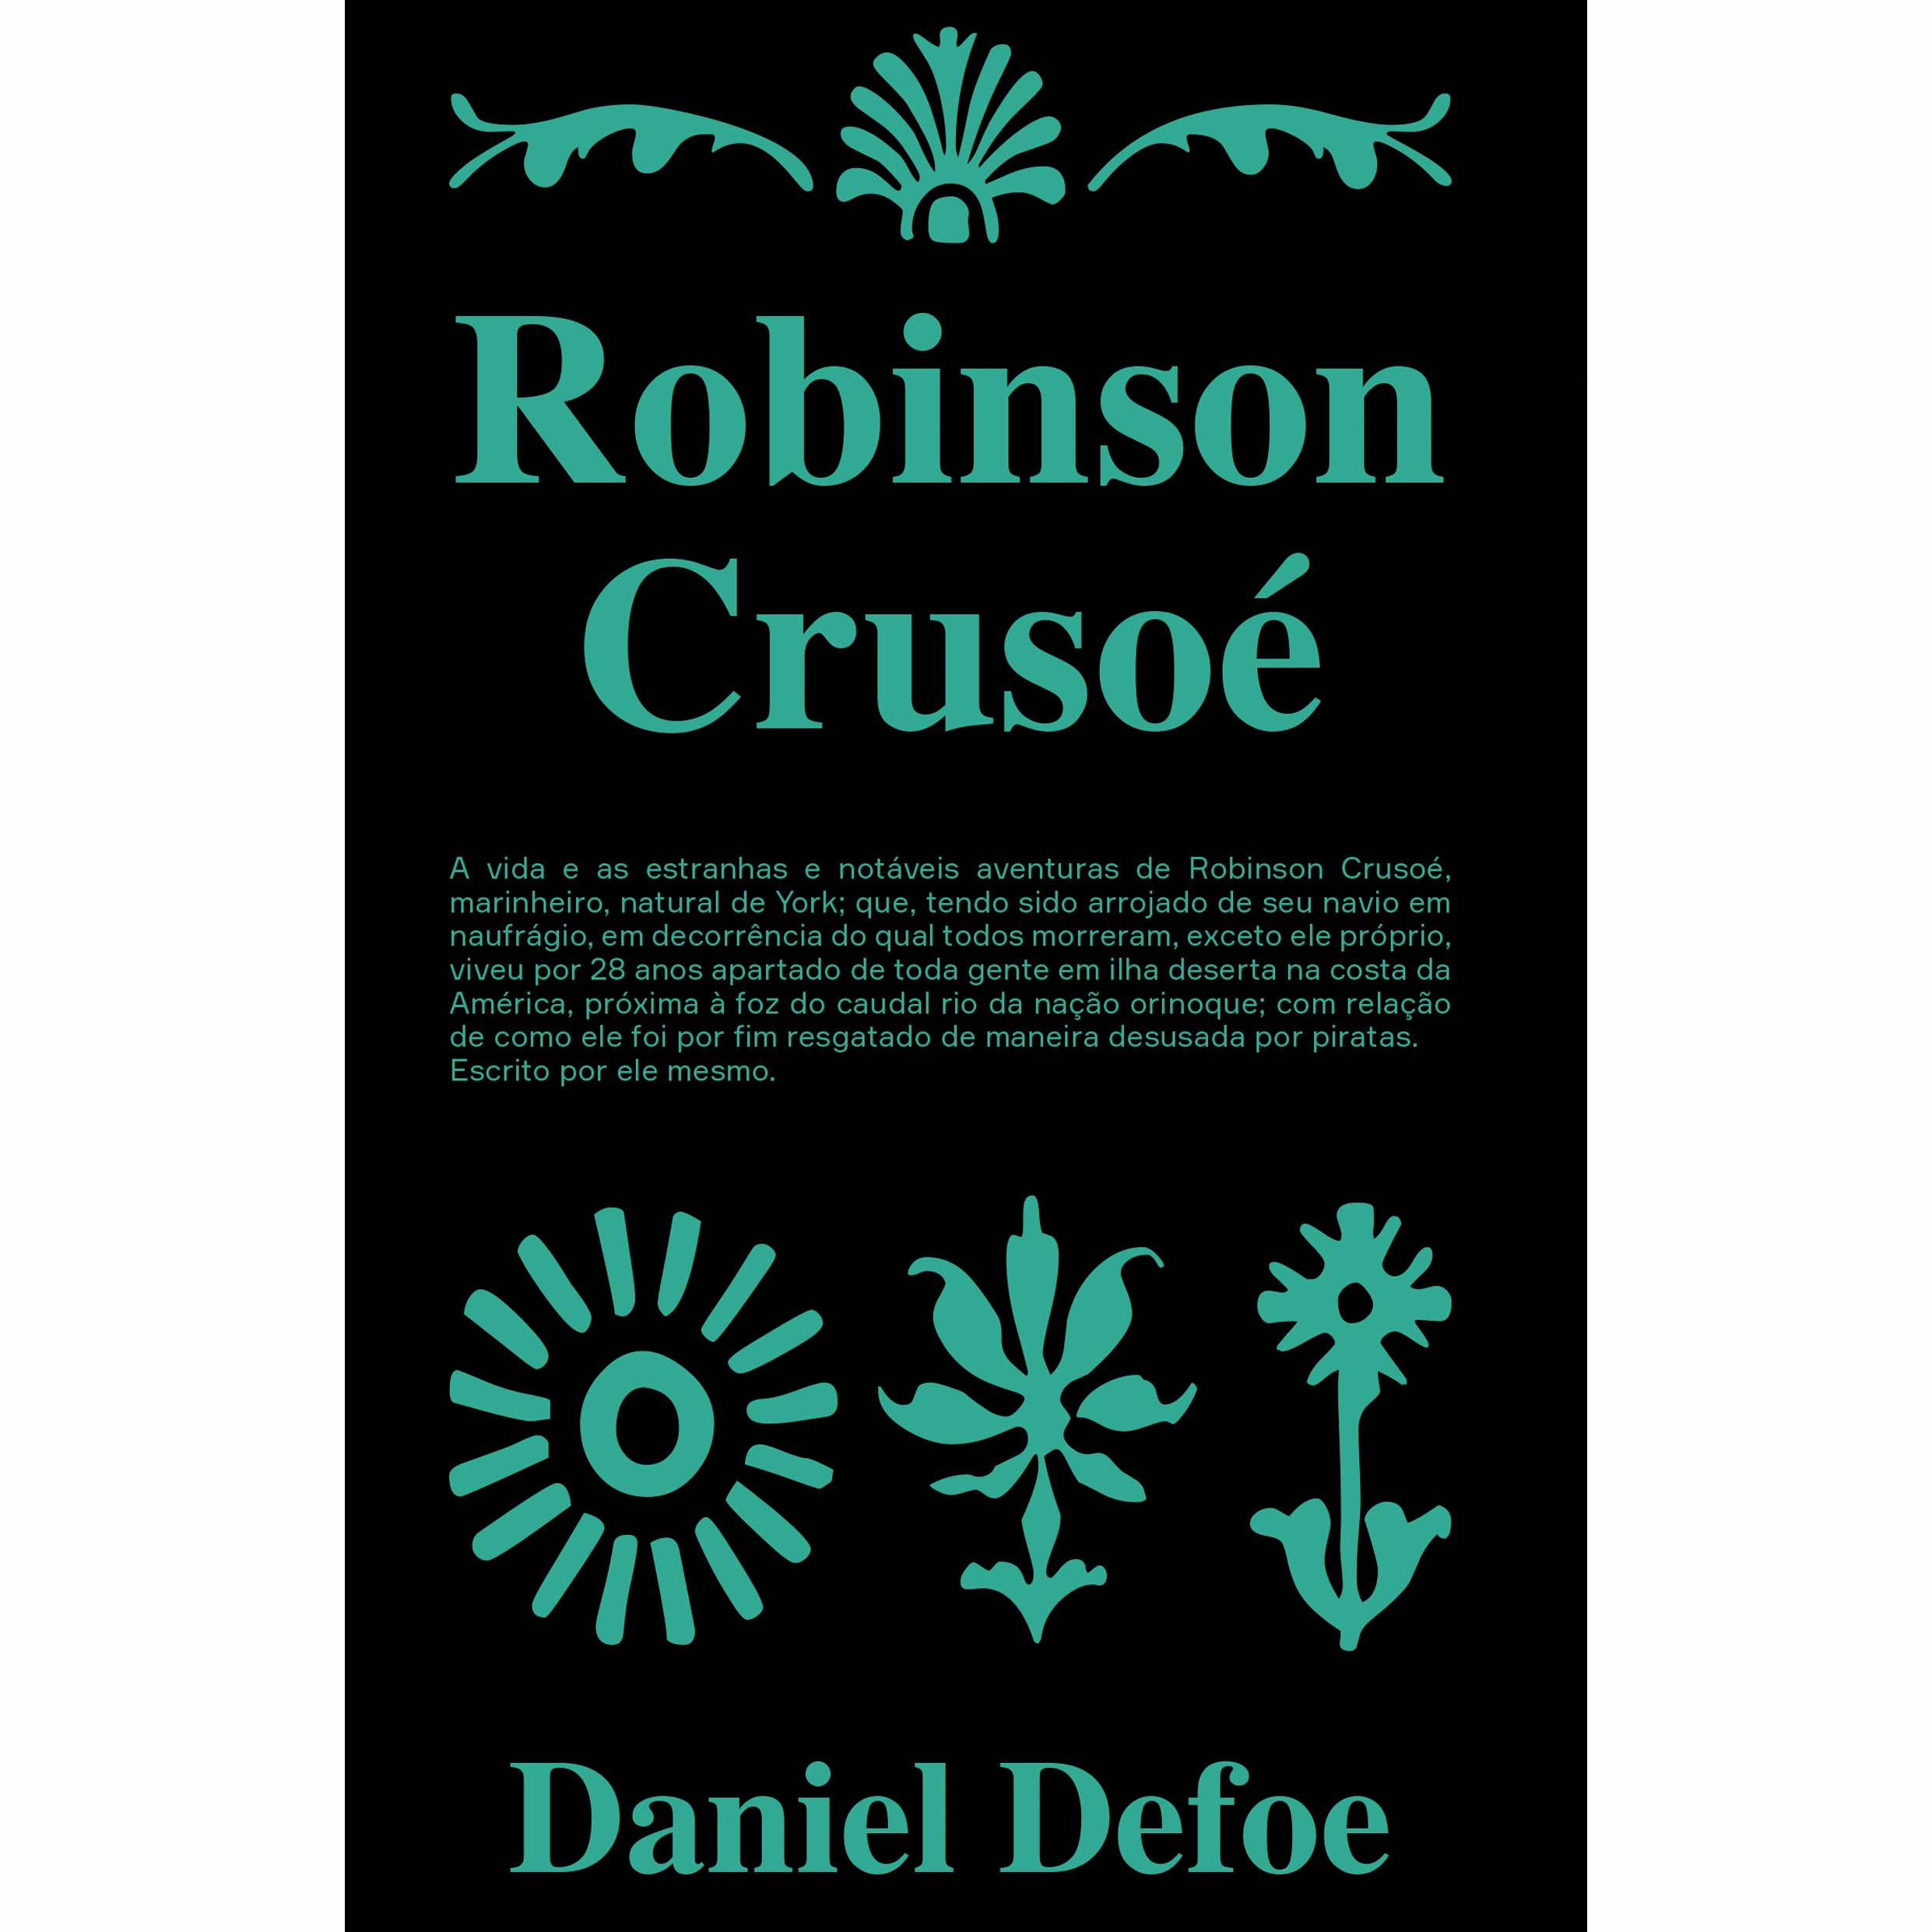
\includegraphics[width=74mm]{./CAPAS/HEDRA_ROBINSON.jpg}
% \end{center}
% \hspace*{-7cm}\hrulefill\hspace*{-7cm}
% \medskip

% \noindent{}Daniel Defoe (1660--1731) escreveu \textit{Robinson Crusoé} em primeira pessoa, livro que segue o modo epistolar de um diário. Publicado durante uma época conhecida por fazer ascender o romance, seus detalhes objetivos influenciaram Herman Melville, em \textit{Moby Dick} (1851).

% O náufrago Robinson Crusoé, que dá nome ao livro, \hlc{é uma espécie de autobiografia fictícia de um homem que passou 28 anos em uma remota ilha tropical encontrando canibais cativos e revoltosos antes de ser resgatado}. Originalmente publicado na forma de folhetins no \textit{The Daily Post}, é um clássico lido em diversas versões --- até mesmo em adaptações infanto-juvenis. É, todavia, uma obra complexa e seus contornos históricos até hoje propõem discussões. 

% \vfill
% \noindent\begin{minipage}[c]{1\linewidth}
% {\small\textbf{
% \hspace*{-.1cm}Editora: Hedra\\
% Título: Robinson Crusoé\\
% Autor: Daniel Defoe\\ 
% ISBN: 978-65-89705-31-4\\
% Páginas: 350 (provisório)\\
% Formato: 13,3x21\,cm\\
% Preço: R\$ 89,00 (provisório)\\
% }}
% \end{minipage}
% \pagebreak

\begin{center}
\hspace*{.5cm}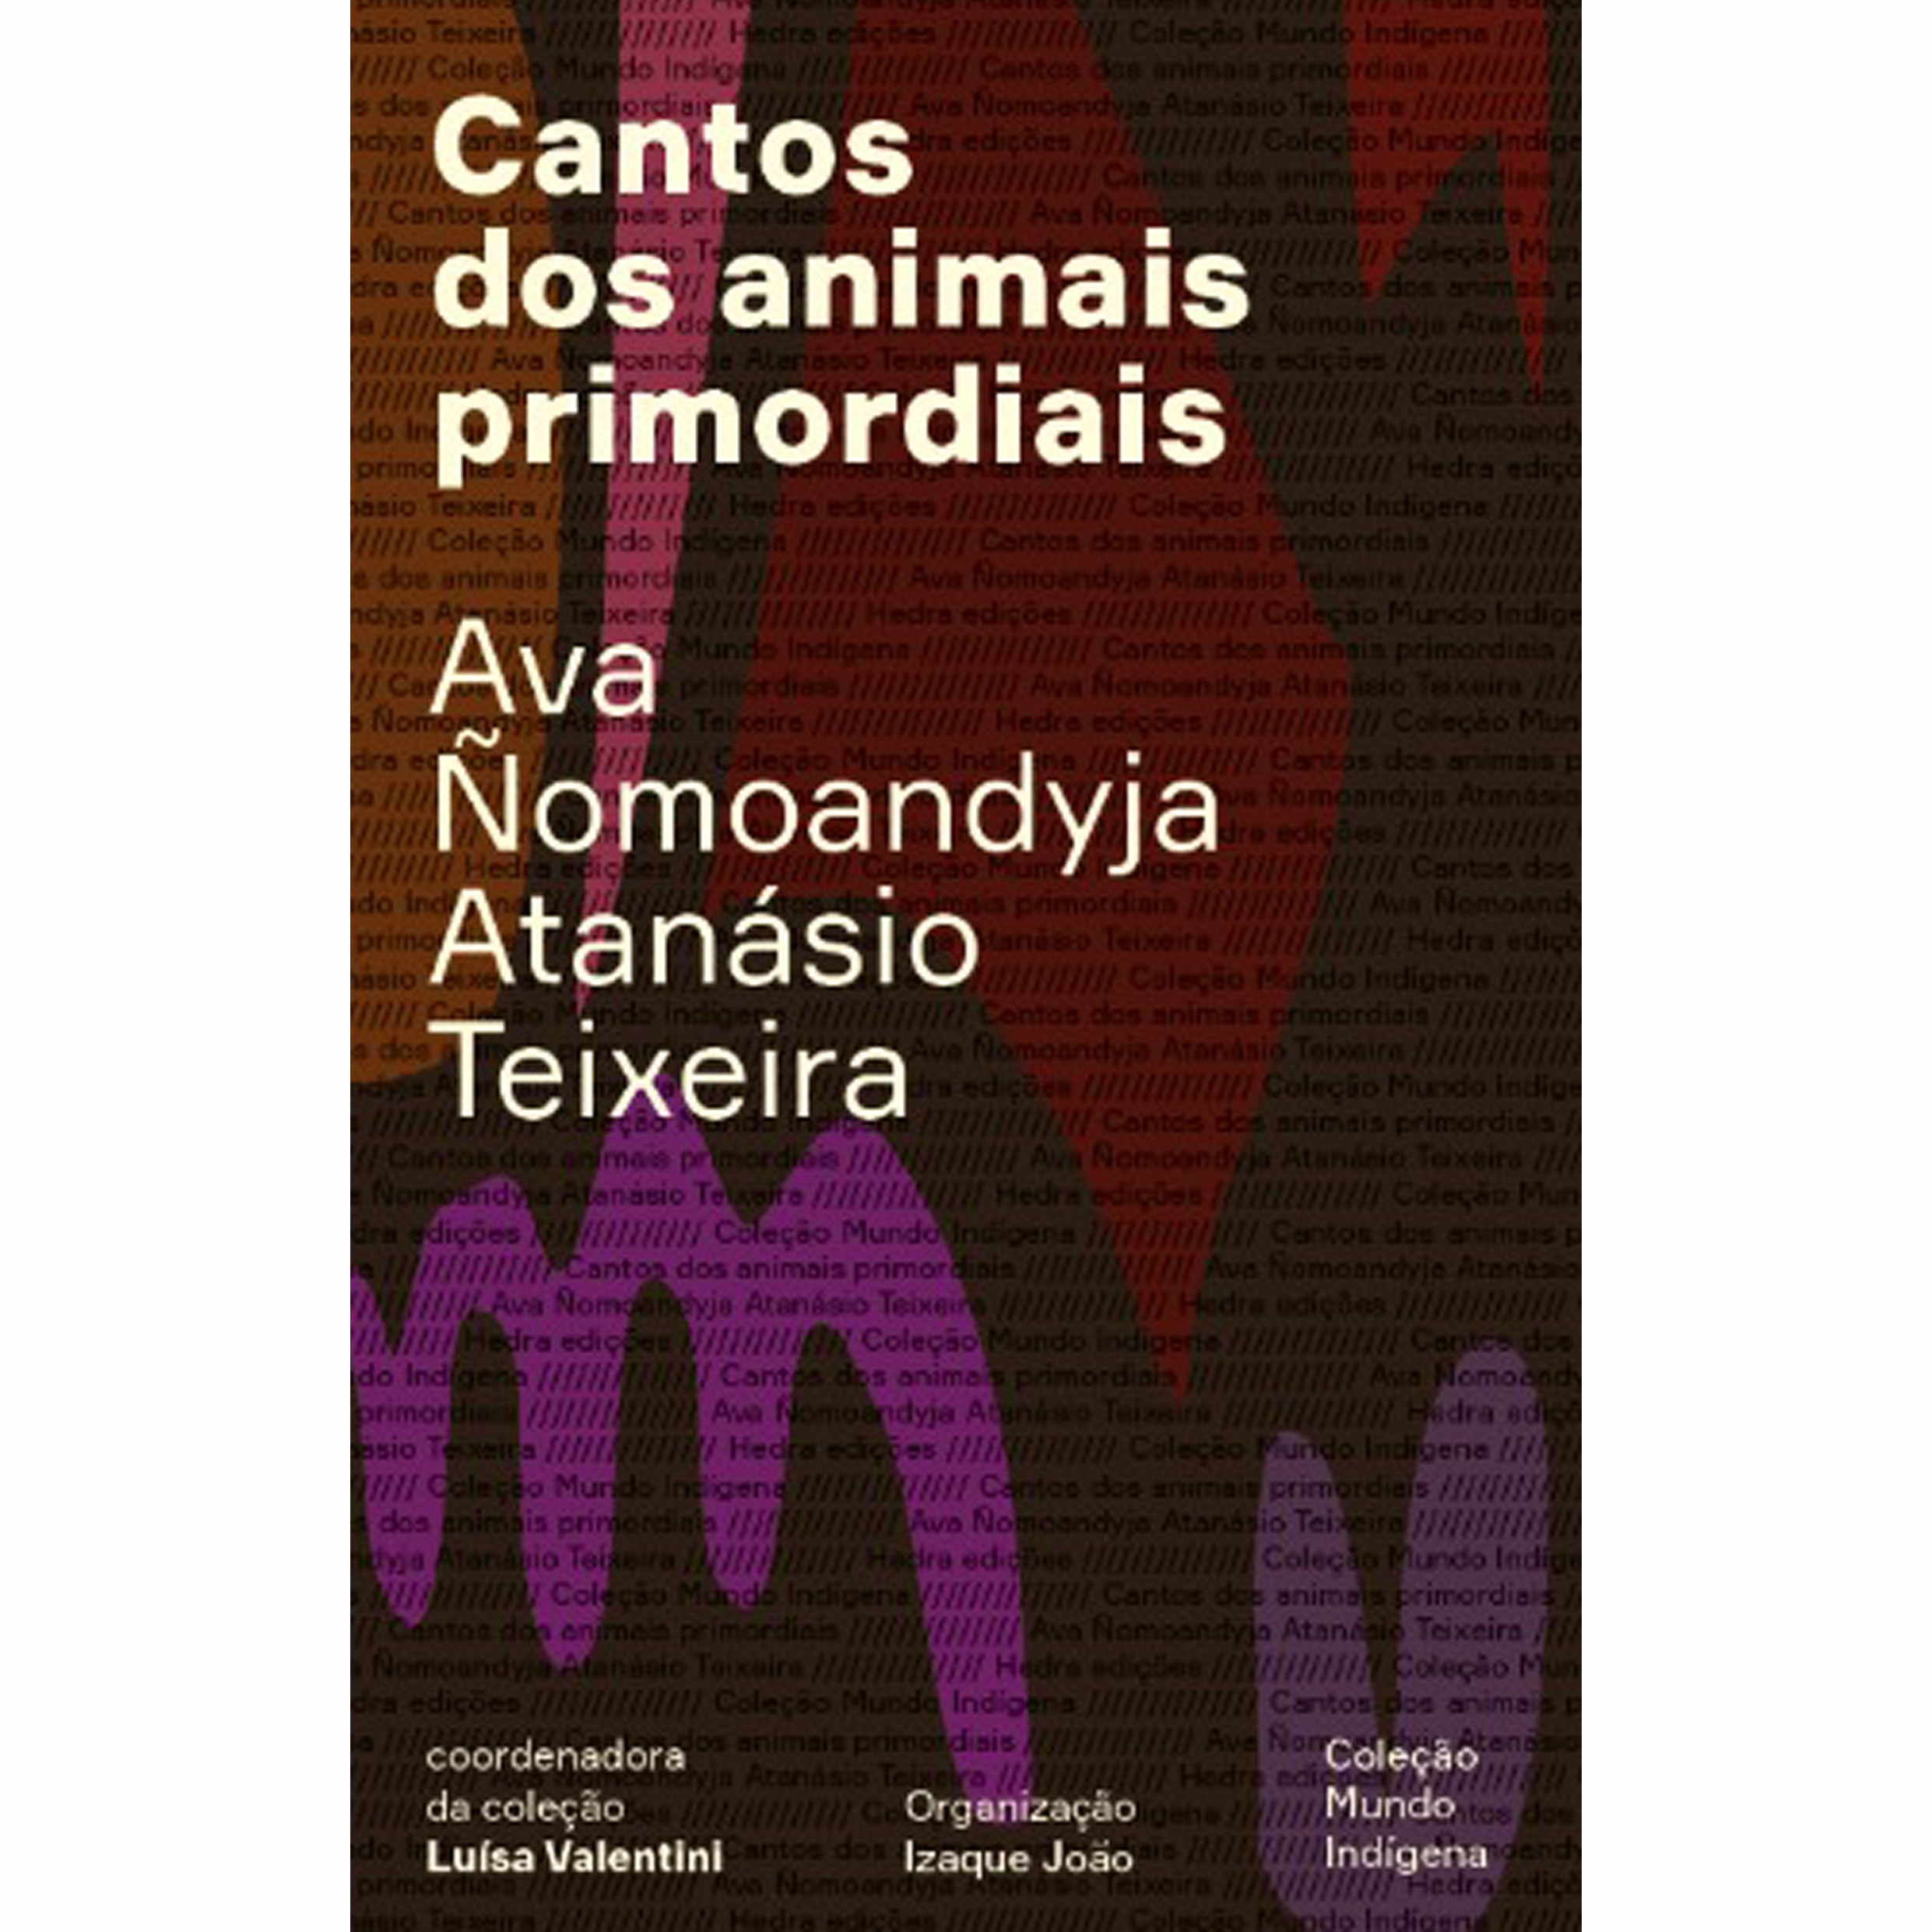
\includegraphics[width=74mm]{./CAPAS/HEDRA_CANTOS.jpg}
\end{center}
\hspace*{-7cm}\hrulefill\hspace*{-7cm}
\medskip

\noindent{}Neste livro são apresentadas \hlc{26 histórias de aves e outros animais da mata, acompanhados pelos cantos \textit{guahu} que cantam sua história desde o princípio dos tempos.} Esses \textit{guahu} fazem parte de um conjunto maior de cantos, rezas e danças dominados por Atanásio Teixeira ou Ava Ñomoandyja, um dos mais prestigiosos xamãs do povo Guarani Kaiowá. As narrativas e explicações que acompanham os cantos foram elaboradas pelo historiador Izaque João, a partir de falas e orientações de Atanásio Teixeira ao longo dos últimos seis anos. 

Os processos de seleção, transcrição e tradução para esta edição bilíngue também foram feitos em diálogo com o xamã e as versões em português dos textos e cantos \textit{guahu} são um exercício de aproximação de suas belas palavras.

\vfill
\noindent\begin{minipage}[c]{1\linewidth}
{\small\textbf{
\hspace*{-.1cm}Editora: Hedra\\
Título: Cantos dos animais primordiais\\
Autor: Ava Ñomoandyja Atanásio Teixeira\\ 
ISBN: 978-65-89705-30-7\\
Páginas: 140\\
Formato: 13,3x21\,cm\\
Preço: R\$ 58,00\\
}}
\end{minipage}
\pagebreak

% \begin{center}
% \hspace*{.5cm}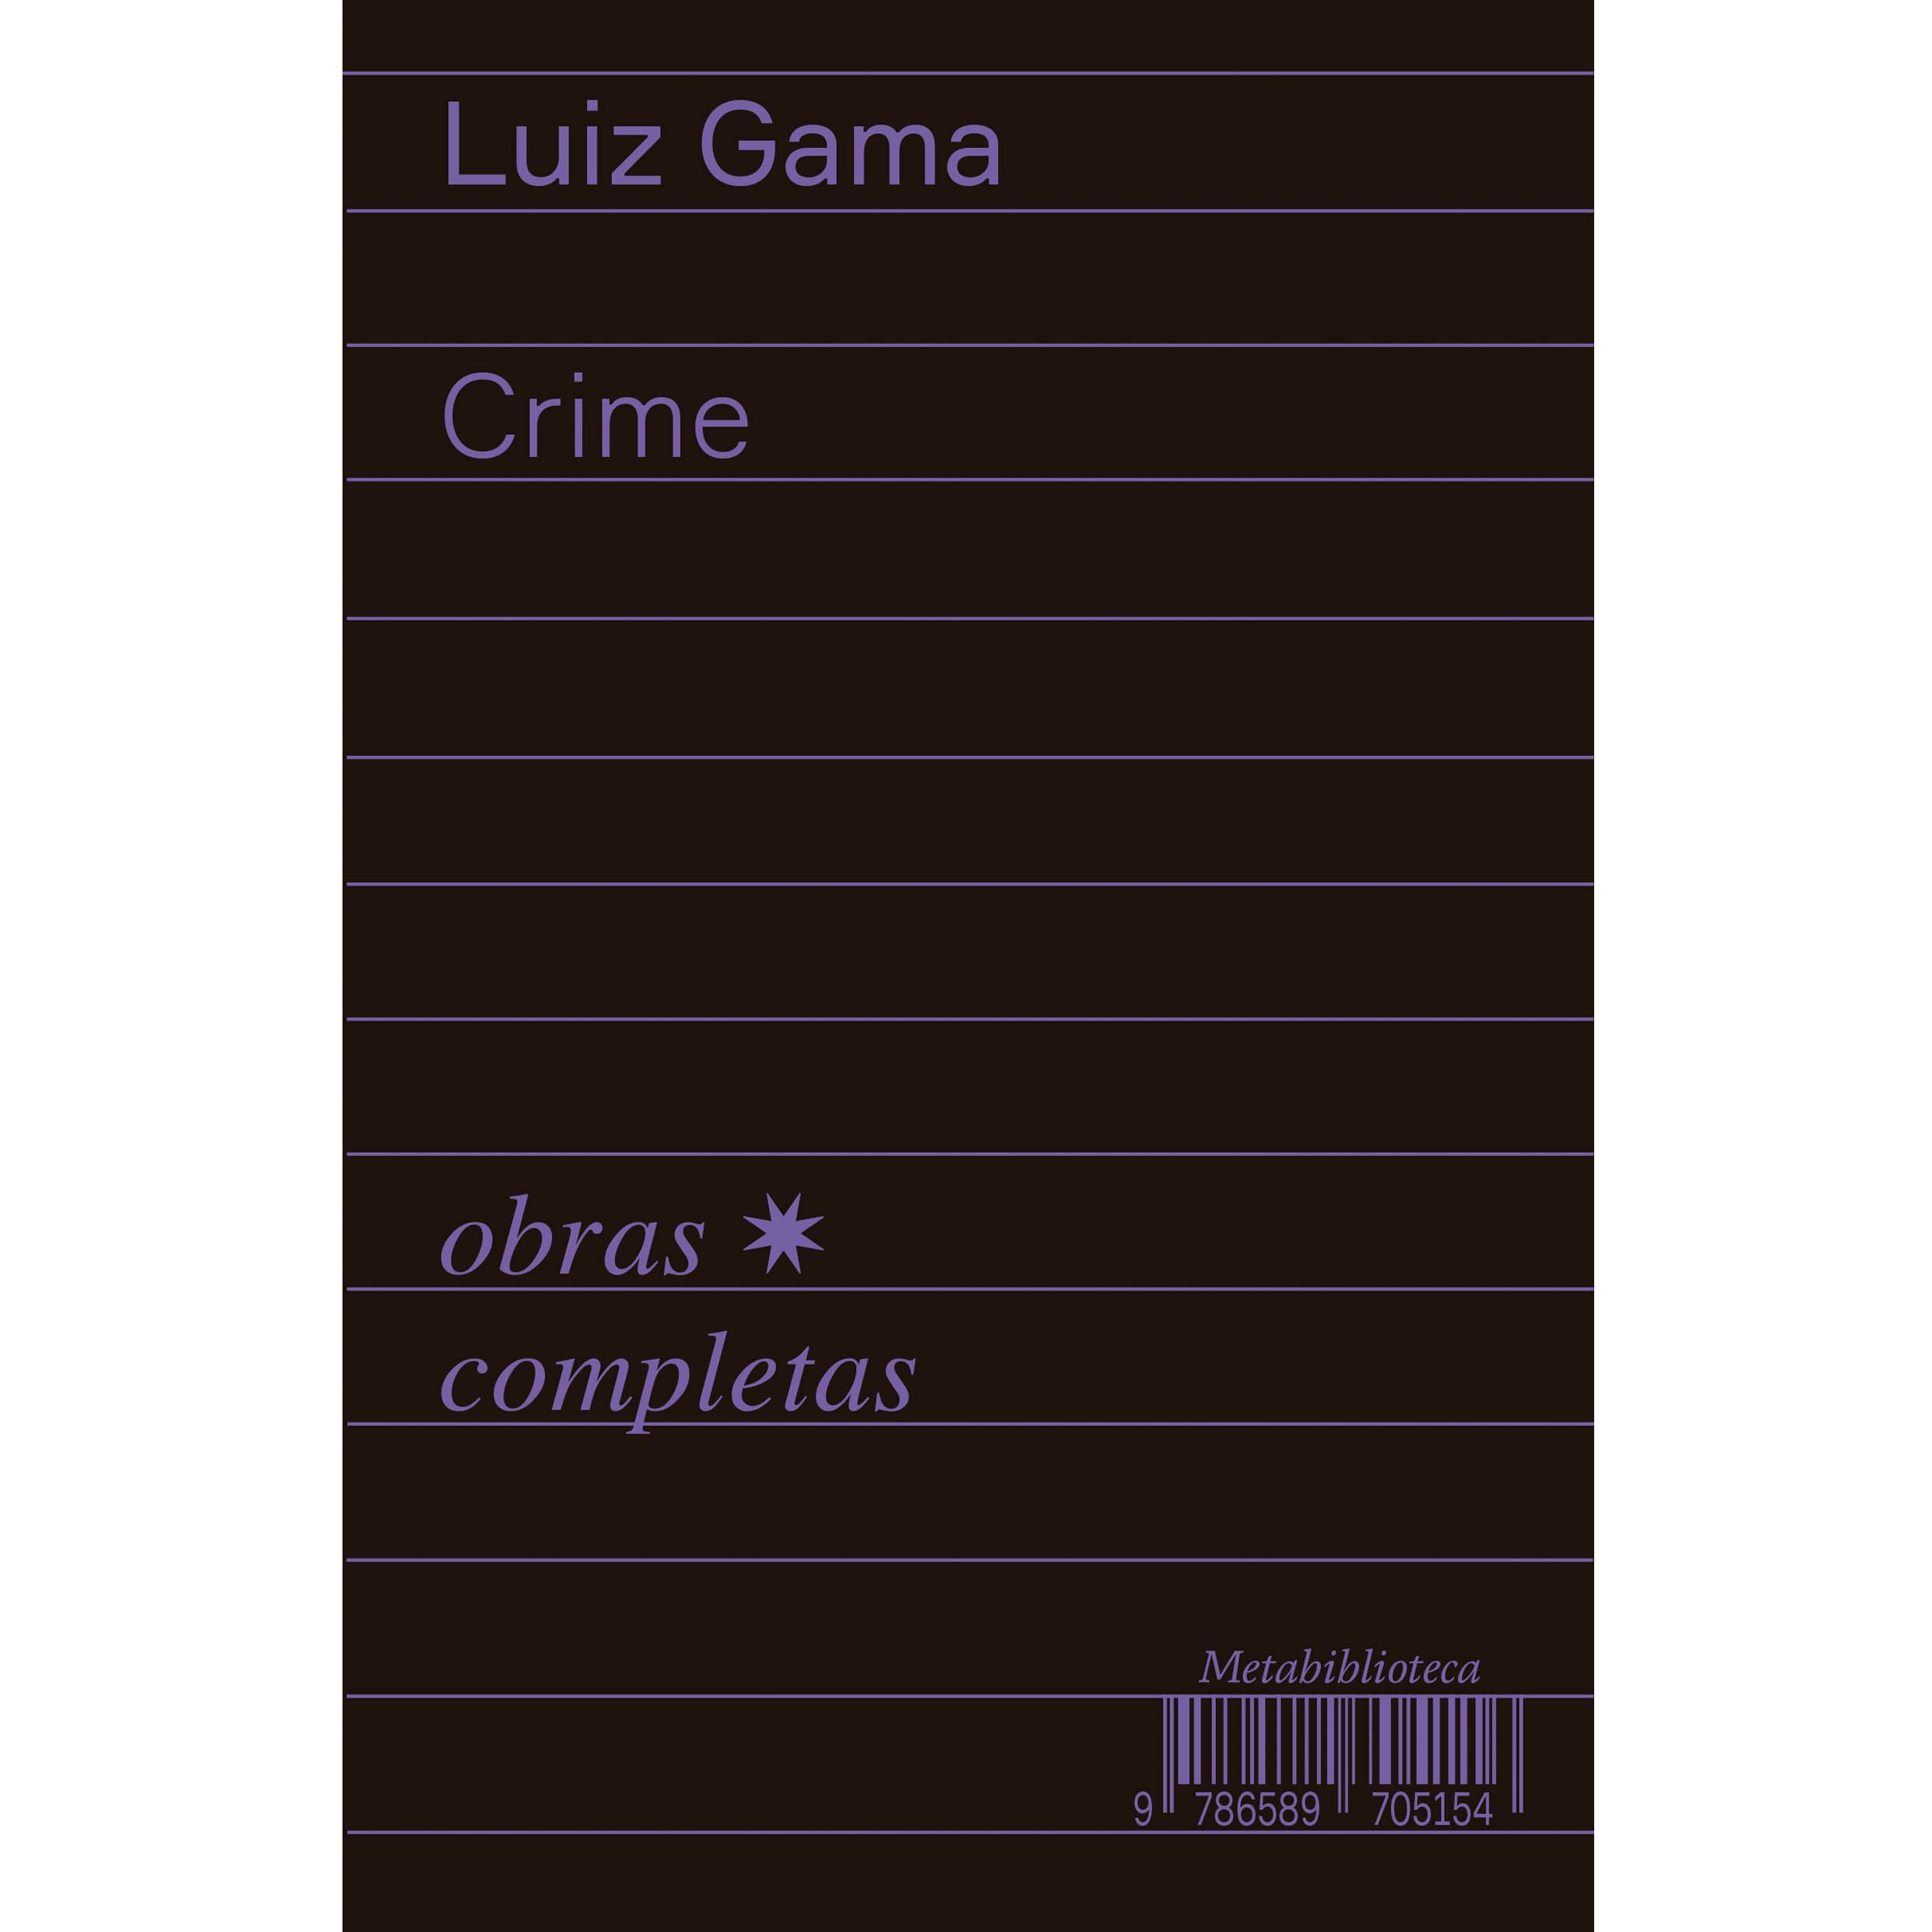
\includegraphics[width=74mm]{./CAPAS/HEDRA_CRIME.jpg}
% \end{center}
% \hspace*{-7cm}\hrulefill\hspace*{-7cm}
% \medskip

% \noindent{}\textit{Crime} apresenta \hlc{a volta de Luiz Gama ao direito a partir de textos que são, em sua maioria, casos criminais: petições de \textit{habeas corpus}, denúncias de violação de direitos de presos e prisões ilegais.} E tornam este livro uma espécie de desenvolvimento do quinto volume, \textit{Direito}. Relacionados à matéria penal e processual penal, \textit{Crime} revela o conhecimento de causa com que interpretava o direito criminal do Brasil. Uma habilidade técnica que outros --- que o chamavam \textit{rábula} --- tentam diminuir, ocultar ou desprezar.

% \textit{Crime} integra as \textit{Obras completas} de Luiz Gama, advogado negro e abolicionista, a serem lançadas em 11 volumes com cerca de 800 escritos --- 600 inéditos ---, revelando as diversas facetas e estilos empregados pelo escritor para advogar pela grande causa de sua vida: a abolição da escravidão e a emancipação negra. Esquecidos em parte por quase dois séculos, os textos foram recuperados pelo pesquisador Bruno Rodrigues de Lima, que passou nove anos localizando-os em arquivos da imprensa e do judiciário de todo o país.

% \vfill
% \noindent\begin{minipage}[c]{1\linewidth}
% {\small\textbf{
% \hspace*{-.1cm}Editora: Hedra\\
% Título: Crime [1877--1879]\\
% Autor: Luiz Gama\\ 
% ISBN: 978-65-89705-15-4\\
% Páginas: Inserir.\\
% Formato: 13,3x21\,cm\\
% Preço: R\$ Inserir.\\
% }}
% \end{minipage}
% \pagebreak

% \begin{center}
% \hspace*{.5cm}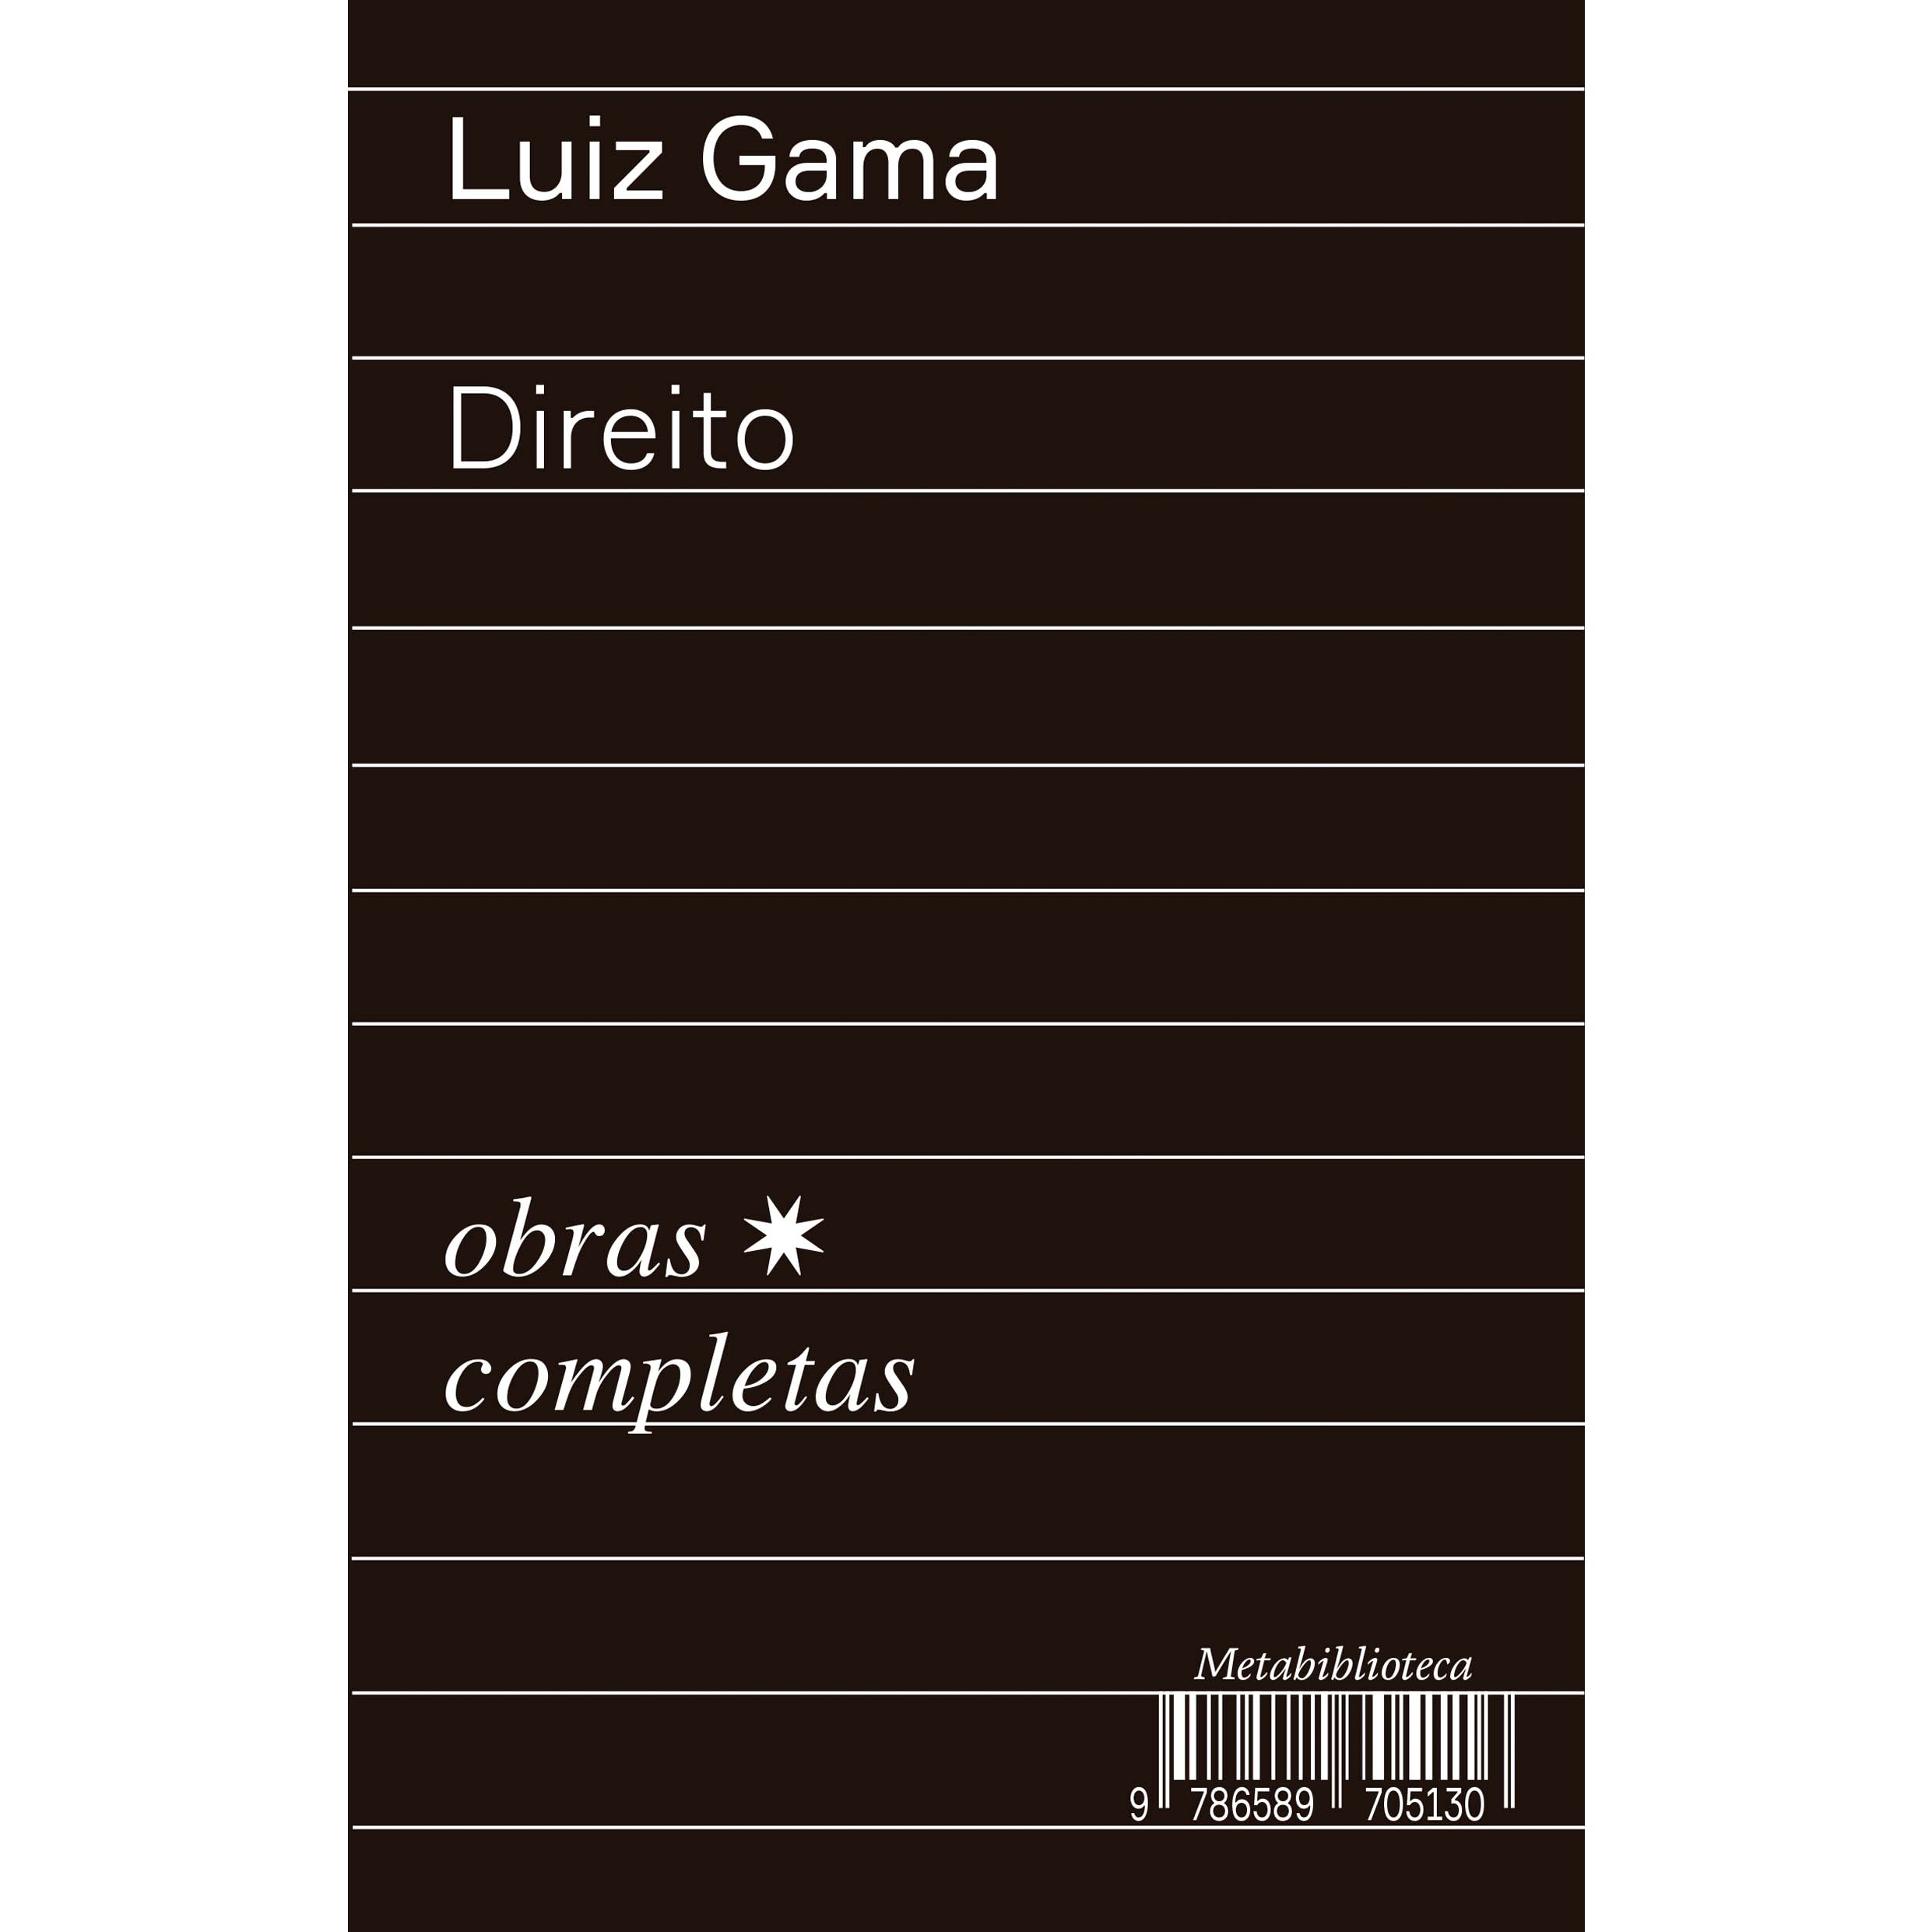
\includegraphics[width=74mm]{./CAPAS/HEDRA_DIREITO.jpg}
% \end{center}
% \hspace*{-7cm}\hrulefill\hspace*{-7cm}
% \medskip

% \noindent{}\textit{Direito} é marcado pela saída de Luiz Gama da polícia e o início de seu percurso como advogado. Este volume reúne sua literatura normativo-pragmática: são textos que podem ser lidos segundo divisões temáticas internas do direito e a partir dos casos concretos. \hlc{A maioria dos textos trata de causas que envolvem escravidão e liberdade, mas Gama também atuou em causas de outras naturezas jurídicas}, eminentemente técnicas, sem lidar com a questão da vida e da morte, o que revela o domínio intelectual do advogado.

% \textit{Direito} integra as \textit{Obras completas} de Luiz Gama, advogado negro e abolicionista, a serem lançadas em 11 volumes com cerca de 800 escritos --- 600 inéditos ---, revelando as diversas facetas e estilos empregados pelo escritor para advogar pela grande causa de sua vida: a abolição da escravidão e a emancipação negra. Esquecidos em parte por quase dois séculos, os textos foram recuperados pelo pesquisador Bruno Rodrigues de Lima, que passou nove anos localizando-os em arquivos da imprensa e do judiciário de todo o país.

% \vfill
% \noindent\begin{minipage}[c]{1\linewidth}
% {\small\textbf{
% \hspace*{-.1cm}Editora: Hedra\\
% Título: Direito [1870--1875]\\
% Autor: Luiz Gama\\ 
% ISBN: 978-65-89705-13-0\\
% Páginas: 400 (provisório)\\
% Formato: 13,3x21\,cm\\
% Preço: R\$ 90,00 (provisório)\\
% }}
% \end{minipage}
% \pagebreak

\vspace*{1.5cm}
\noindent{}{\nohyphens{\LARGE{Casamento e amor}}}
\bigskip

\hfill{}\scalebox{.8}{EMMA GOLDMAN}
\bigskip
\bigskip
\bigskip

\begin{multicols}{2}
\noindent{}A concepção popular sobre o casamento e o amor é a de que estes dois
termos são sinônimos, que surgem pelas mesmas razões e abarcam as mesmas
necessidades humanas. Tal como ocorre com a maioria das concepções
populares, isso não se baseia em fatos reais, mas tão somente em
superstições.

Casamento e amor não têm nada em comum; eles estão tão longe um do outro
quanto dois polos; são, na verdade, antagônicos entre si. Não há dúvidas
de que alguns casamentos resultam do amor. No entanto, não porque o
amor só pudesse se fazer valer sob o casamento, e sim, muito mais,
porque apenas poucas pessoas podem superar as convenções. Há, hoje em
dia, um grande número de homens e mulheres para quem o casamento nada
mais é do que uma farsa, não obstante se submetam a ele em prol da
opinião pública. Ainda que, para todos os efeitos, seja verdade que
alguns casamentos se baseiam no amor, tal como é igualmente verdadeiro
que, em certos casos, o amor continua na vida de casado, mantenho
a posição de que isso se dá independentemente do casamento, e
não por causa dele.

Por outro lado, é absolutamente falso que o amor resulte do casamento.
Em raras ocasiões, pode"-se ouvir casos miraculosos acerca de casais que
se apaixonam completamente um pelo outro após o casamento, mas com um
exame mais minucioso se descobrirá que se trata apenas de mero ajuste ao
que é inevitável. Certamente, acostumar"-se um ao outro é bem diferente
da espontaneidade, da intensidade e da beleza do amor, elementos sem os
quais a intimidade do casamento demonstrou"-se degradante tanto para a
mulher quanto para o homem.

\vspace{\baselineskip}
{\small\fakereceipt{
\noindent{}Separados por um muro intransponível de superstição, costumes e hábitos,
o casamento não tem o potencial de desenvolver a intimidade e o
respeito mútuos, sem os quais toda união está fadada ao fracasso.}}
\vspace{\baselineskip}

O casamento é, antes de tudo, um acordo econômico, uma apólice de
seguro. Difere de um seguro de vida propriamente dito apenas porque é
mais compulsório, mais exigente. Seu retorno é insignificante quando
comparado aos investimentos. Ao fazer uma apólice de seguro, paga"-se por
ela em dólares e centavos, sempre tendo a liberdade de suspender os
pagamentos. Se, no entanto, o abono de uma mulher for um marido, ela
paga por ele com o seu nome, sua privacidade, seu amor"-próprio, sua vida
como um \textit{até que a morte vos separe}. Além disso a apólice
casamento a condena a uma dependência por toda a vida, ao parasitismo, a
uma completa inutilidade seja individual ou social. Os homens também
pagam a sua taxa, mas como a sua esfera é mais ampla, o casamento não
limita tanto quanto no caso da mulher. Ele sente as suas correntes mais
no sentido econômico.

Assim, o lema de Dante sobre a porta do Inferno se aplica com igual força
ao casamento: ``Deixai toda esperança, vós que entrais!''

Que o casamento é um fracasso ninguém, exceto os mais
estúpidos, poderá negar. Um breve relance nas estatísticas do divórcio é
suficiente para que se constate quão amargo um casamento fracassado é. Argumentos
estereotipados e típicos de filisteus de que tal aumento se deve à frouxidão
das leis do divórcio e à crescente liberdade das mulheres não dão conta
do fato de que: em primeiro lugar, um em cada 12 casamentos termina em
divórcio; em segundo, que desde 1870, os divórcios aumentaram de 28 para
73 por 100.000 habitantes; em terceiro, que, desde 1867, o adultério,
como motivo para o divórcio, aumentou 270,8\%; e em quarto, que a
deserção do cônjuge aumentou 369,8\%.

Assomado a esses dados alarmantes, há uma vasta quantidade de material
dramático e literário que promove a elucidação do assunto. Robert
Herrick, no seu \textit{Together}; Pinero, em \textit{Mid"-Channel}; Eugene
Walter, em \textit{Paid in full}, e muitos outros escritores discutem a
esterilidade, a monotonia, a sordidez, numa palavra, a inadequação do
casamento para a harmonia e a compreensão.

Qualquer estudioso das questões sociais que seja capaz de pensar não irá
se contentar com a desculpa popular e superficial, em geral, dada a este fenômeno. Ele
terá de se aprofundar na vida real dos sexos para descobrir por que o
casamento é tão desastroso.

Edward Carpenter diz que por trás de todo casamento encontra"-se o
contexto de vida dos dois sexos; um contexto tão diferente um do outro
que homens e mulheres têm de permanecer estranhos um ao outro.
Separados por um muro intransponível de superstição, costumes e hábitos,
o casamento não tem o potencial de desenvolver a intimidade e o
respeito mútuos, sem os quais toda união está fadada ao fracasso.

Henrik Ibsen, que odiava todas as hipocrisias sociais, foi, provavelmente,
o primeiro a entender essa grande verdade. Nora deixa o marido,
não --- como defendem os críticos estúpidos --- porque ela estivesse
cansada das suas responsabilidades ou porque ansiasse pelos direitos da
mulher, mas, sim, porque chegou à compreensão de que viveu com um
estranho por oitos anos, com quem teve filhos. Pode haver algo mais
humilhante, mais degradante do que uma proximidade, ao longo de uma
vida, entre dois estranhos?\footnote{Referência à peça \textit{Casa de bonecas}, cuja publicação e estreia, em 1879, garantiu o primeiro sucesso internacional de Ibsen.} Não há necessidade de a mulher saber
qualquer coisa sobre o marido, exceto a sua renda. E o que o homem
precisa saber sobre a mulher que não seja se ela possui uma aparência
atraente? Ainda não superamos o mito teológico de que a mulher não tem
alma, que ela é um mero apêndice do homem, feita da costela apenas para
a conveniência do cavalheiro em questão, que de tão forte teme a sua
própria sombra.\label{ref7}

Talvez a má qualidade da matéria"-prima com que a mulher foi feita seja a
responsável pela sua inferioridade. De qualquer forma, a mulher não tem
alma --- o que haveria, então, de se saber sobre ela? Além disso, quanto
menos alma uma mulher tiver, mais adequada estará à condição de esposa,
mais prontamente irá se deixar absorver em seu marido. É a aceitação
servil da superioridade do homem que tem mantido a instituição casamento
aparentemente intacta por tanto tempo. Agora que a mulher está se
tornando ela mesma, agora que ela está realmente se tornando consciente
de si como um ser independente das graças do seu mestre, a instituição
sagrada do casamento gradualmente está sendo solapada, e nenhum montante
de lamentação sentimental pode modificar isso.

Desde a infância, é dito, praticamente, a todas as garotas que o
casamento é o seu objetivo final; portanto seu treinamento e educação
devem ser dirigidos com vistas a esse fim. Tal como um animal mudo que é
posto na engorda para o seu conseguinte abate, ela é preparada para o
casamento. No entanto, por mais estranho que pareça, é"-lhe permitido
saber muito menos sobre a sua função como esposa e mãe do que a um
artesão comum sobre o seu ofício. Para uma garota respeitável, é\label{artesao}
indecente e sujo saber qualquer coisa sobre a relação matrimonial. Ora,
ante a inconsistência de tal respeitabilidade, necessita"-se do voto
de casamento para tornar algo que é sujo em um arranjo tão puro e tão
sagrado, que ninguém ousará questionar ou criticar.
Essa é precisamente a atitude de qualquer defensor mediano do
casamento. A futura mãe e esposa é mantida em completa ignorância acerca do seu
único recurso na arena competitiva: o sexo. Assim, ela adentra relações
de longo prazo com um homem apenas para, posteriormente, vir a se sentir
chocada, rechaçada, indignada para além de qualquer medida com o mais
natural e saudável dos instintos, o sexo. Pode"-se dizer com certeza que
uma grande porcentagem da infelicidade, miséria, angústia e sofrimento
físico do casamento se deve à ignorância criminosa em questões sexuais
--- ignorância que é exaltada como uma grande virtude. Não é exagero
dizer que mais do que um lar foi destruído, devido a esse fato
deplorável.

Se, no entanto, a mulher se tornar livre e grande o suficiente para
aprender os mistérios do sexo sem a sanção do Estado e da Igreja, ela
será condenada como absolutamente inadequada para se tornar a esposa de
um \textit{bom homem} --- bondade que consiste numa cabeça vazia e muito
dinheiro. Pode haver algo mais ultrajante do que a ideia de que uma
mulher saudável e adulta, cheia de vida e paixão, deve negar as demandas
da natureza, deve subjugar o seu mais intenso desejo, minar sua saúde,
quebrar seu espírito, atrofiar sua visão, abster"-se da profundidade
e da glória da experiência sexual até que um \textit{bom homem} apareça
para tomá-la como esposa? É exatamente isso o que o casamento significa.
Como tal arranjo poderia terminar de outra forma que não em fracasso?
Este é um dos fatores, certamente não o menos importante, que
diferencia o casamento do amor.

\bigskip
\noindent{}\textcolor{gray}{\footnotesize\slsc{\textls[-15]{Excerto do capítulo ``Casamento e amor'' do livro \textit{Sobre anarquismo, sexo e casamento}, texto de 1910.}}}
\end{multicols}

\pagebreak
\pagestyle{hedracat}
\begin{multicols}{2}
\begin{enumerate}
\raggedright\nohyphens{
\item A sociedade de controle \textbf{Joyce Souza, Rodolfo Avelino, Sérgio Amadeu da Silveira}
\item O contador de histórias e outros textos \textbf{Walter Benjamin}
\item Diário parisiense e outros escritos \textbf{Walter Benjamin}
\item Rashômon e outros contos \textbf{Akutagawa}
\item A linguagem fascista \textbf{Carlos Piovezani, Emilio Gentile}
\item Teogonia \textbf{Hesíodo}
\item Liberdade (1880-1882) \textbf{Luiz Gama}
\item Poesia completa \textbf{Orides Fontela}
\item Sobre verdade e mentira \textbf{Friedrich Nietzsche}
\item A volta do parafuso \textbf{Henry James}
\item Democracia (1866-1869) \textbf{Luiz Gama}
\item Trabalhos e os dias \textbf{Hesíodo}
\item Deus e o Estado \textbf{Mikhail Bakunin}
\item Hino a Afrodite e outros poemas \textbf{Safo de Lesbos}
\item O princípio anarquista e outros ensaios \textbf{Piotr Alekseievitch Kropotkin}
\item Pandemia e anarquia \textbf{Edson Passetti, João da Mata, José Maria Carvalho Ferreira}
\item Lugar de negro, lugar de branco? \textbf{Douglas Rodrigues Barros}
\item O indivíduo, a sociedade e o Estado e outros ensaios \textbf{Emma Goldman}
\item Machismo, racismo, capitalismo identitário \textbf{Pablo Polese}
\item Dicionário de mitologia nórdica \textbf{Johnni Langer}
\item Freud e o patriarcado \textbf{Léa Silveira, Alessandra Martins Parente}
\item Dicionário de história e cultura da era Viking \textbf{Johnni Langer} 
\item O princípio do Estado e outros ensaios \textbf{Mikhail Bakunin}
\item Sobre a utilidade e a desvantagem da história para a vida \textbf{Friedrich Nietzsche}
\item Ode sobre a melancolia e outros poemas \textbf{John Keats}
\item O chamado de Cthulhu \textbf{H. P. Lovecraft}
\item Saga dos Volsungos \textbf{Anônimo}
\item Os sofrimentos do jovem Werther \textbf{Johann Wolfgang Von Goethe}
\item Memórias do subsolo \textbf{Fiódor Dostoiévski}
\item A monadologia e outros textos \textbf{Gottfried Leibniz}
}
\end{enumerate}
\end{multicols}

\pagebreak
